\documentclass[aspectratio=169]{beamer}

\usetheme[progressbar=frametitle]{metropolis}
\usepackage{appendixnumberbeamer}
\usepackage{booktabs}
\usepackage[scale=2]{ccicons}
\usepackage{xspace}
\usepackage{caption}
\usepackage{subcaption}
\usepackage{amsmath, amssymb}

\title{Лекция 0: Вводная}
\subtitle{История, необходимые для понимания термины и мемы}
\date{11 января 2020}

\begin{document}

\maketitle

\begin{frame}{История вопроса}
    \begin{figure}
        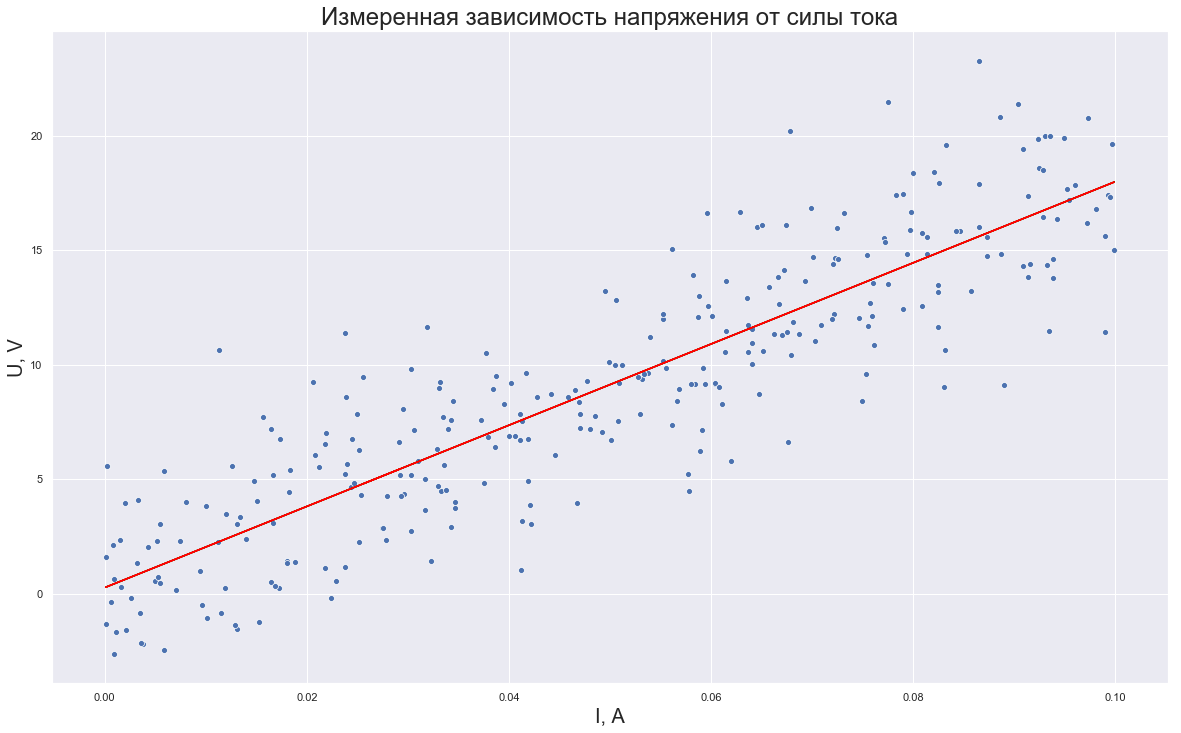
\includegraphics[width=\linewidth]{graphs/fig1.png}
        \caption{80 лет истории исследований AI}
    \end{figure}
\end{frame}

\begin{frame}{История вопроса}
    \begin{columns}
        \begin{column}{0.48\linewidth}
            \begin{figure}
                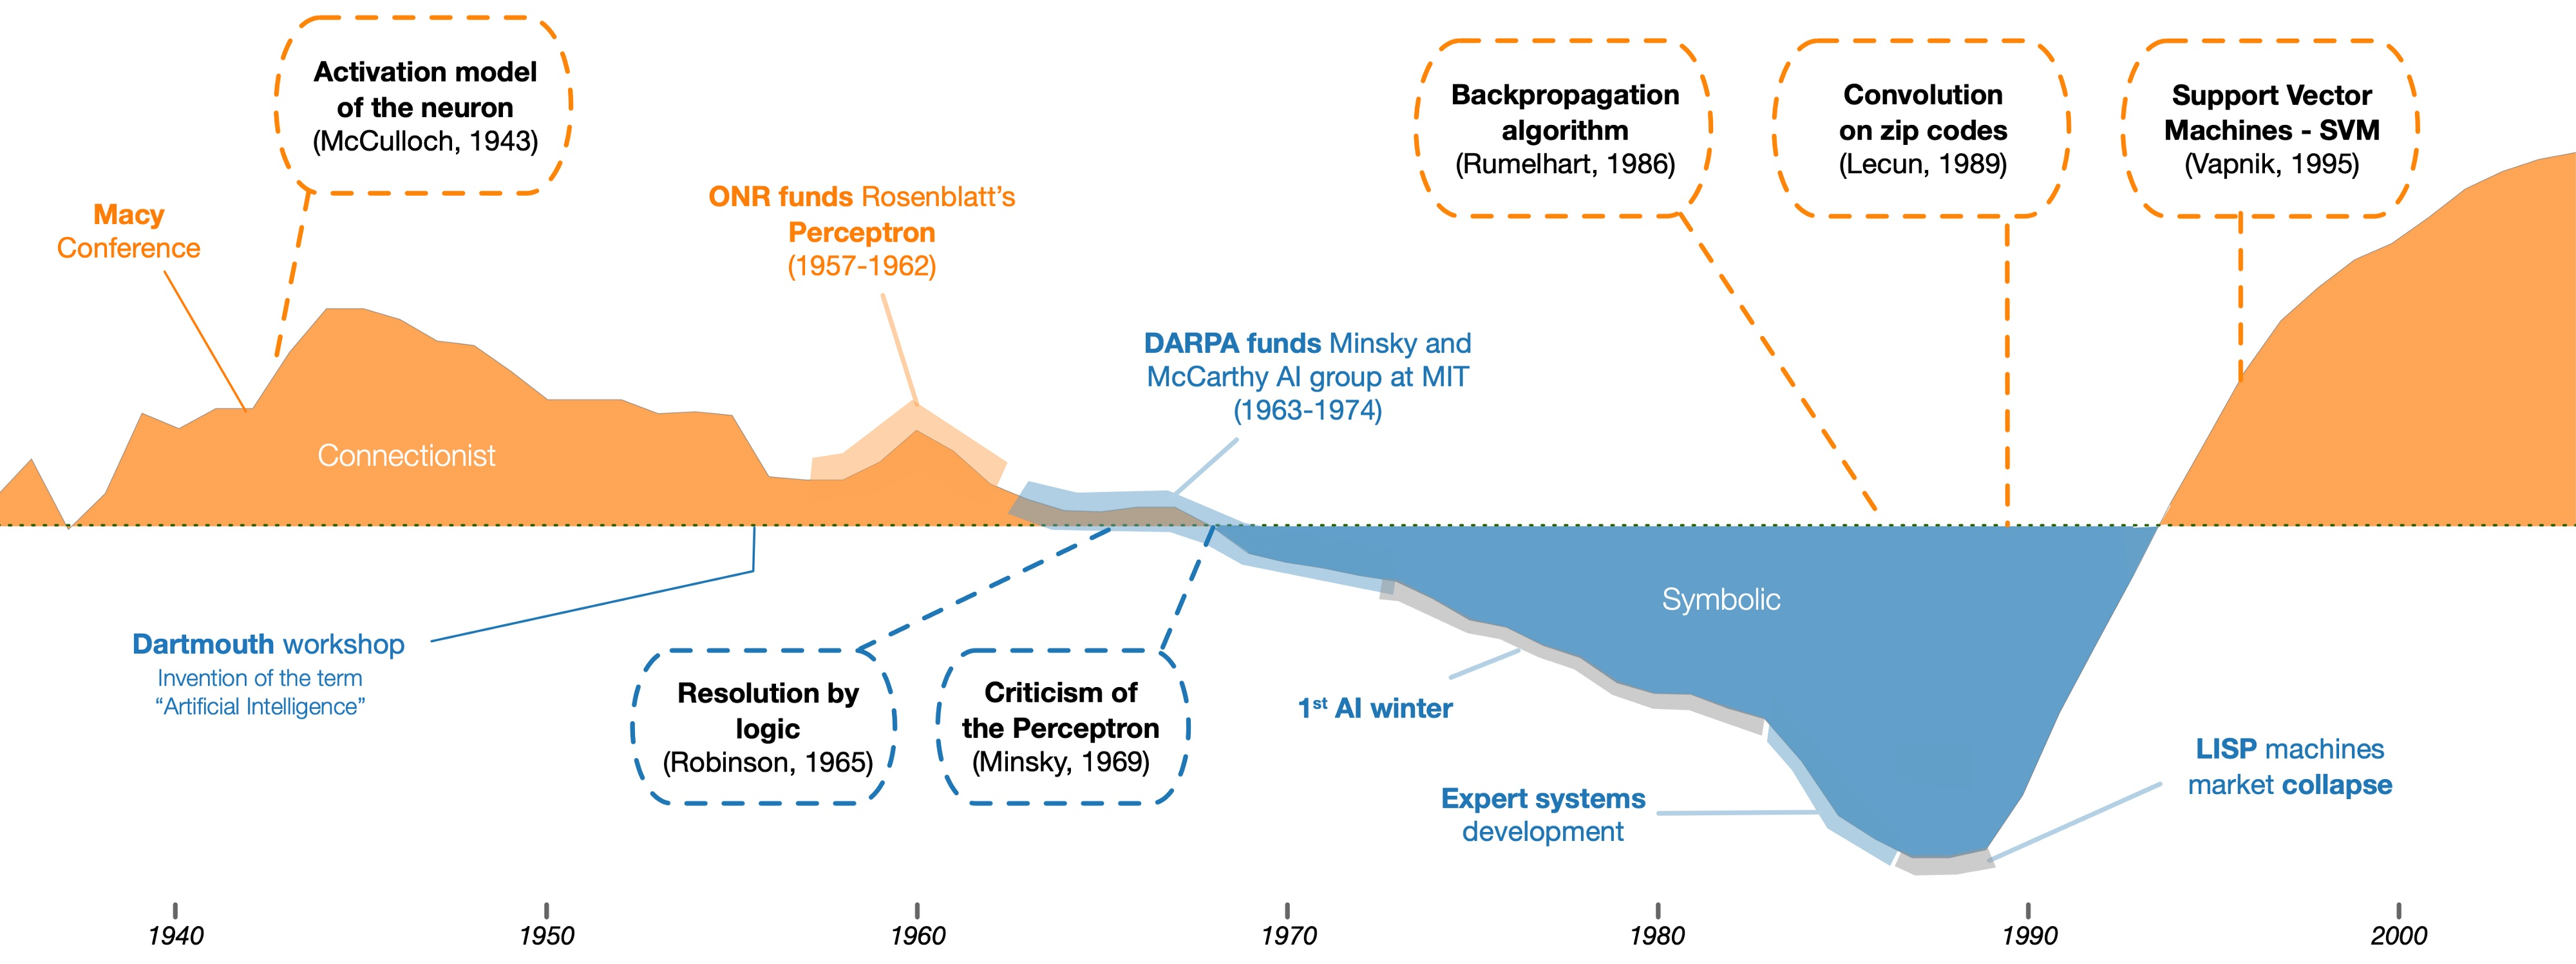
\includegraphics[width=0.9\linewidth]{graphs/fig2.jpg}
                \caption{Ожидание}
            \end{figure}
        \end{column}
        \pause{}
        \begin{column}{0.48\linewidth}
            \begin{figure}
                \includegraphics[width=0.49\linewidth]{graphs/fig2_1.png}
                \caption{Реальность}
            \end{figure}
        \end{column}
    \end{columns}
\end{frame}

\begin{frame}{Задача классификации изображений}
    \centering
    \LARGE
    Что такое классификация изображений?
\end{frame}

\begin{frame}{Задача классификации изображений}
    \centering
    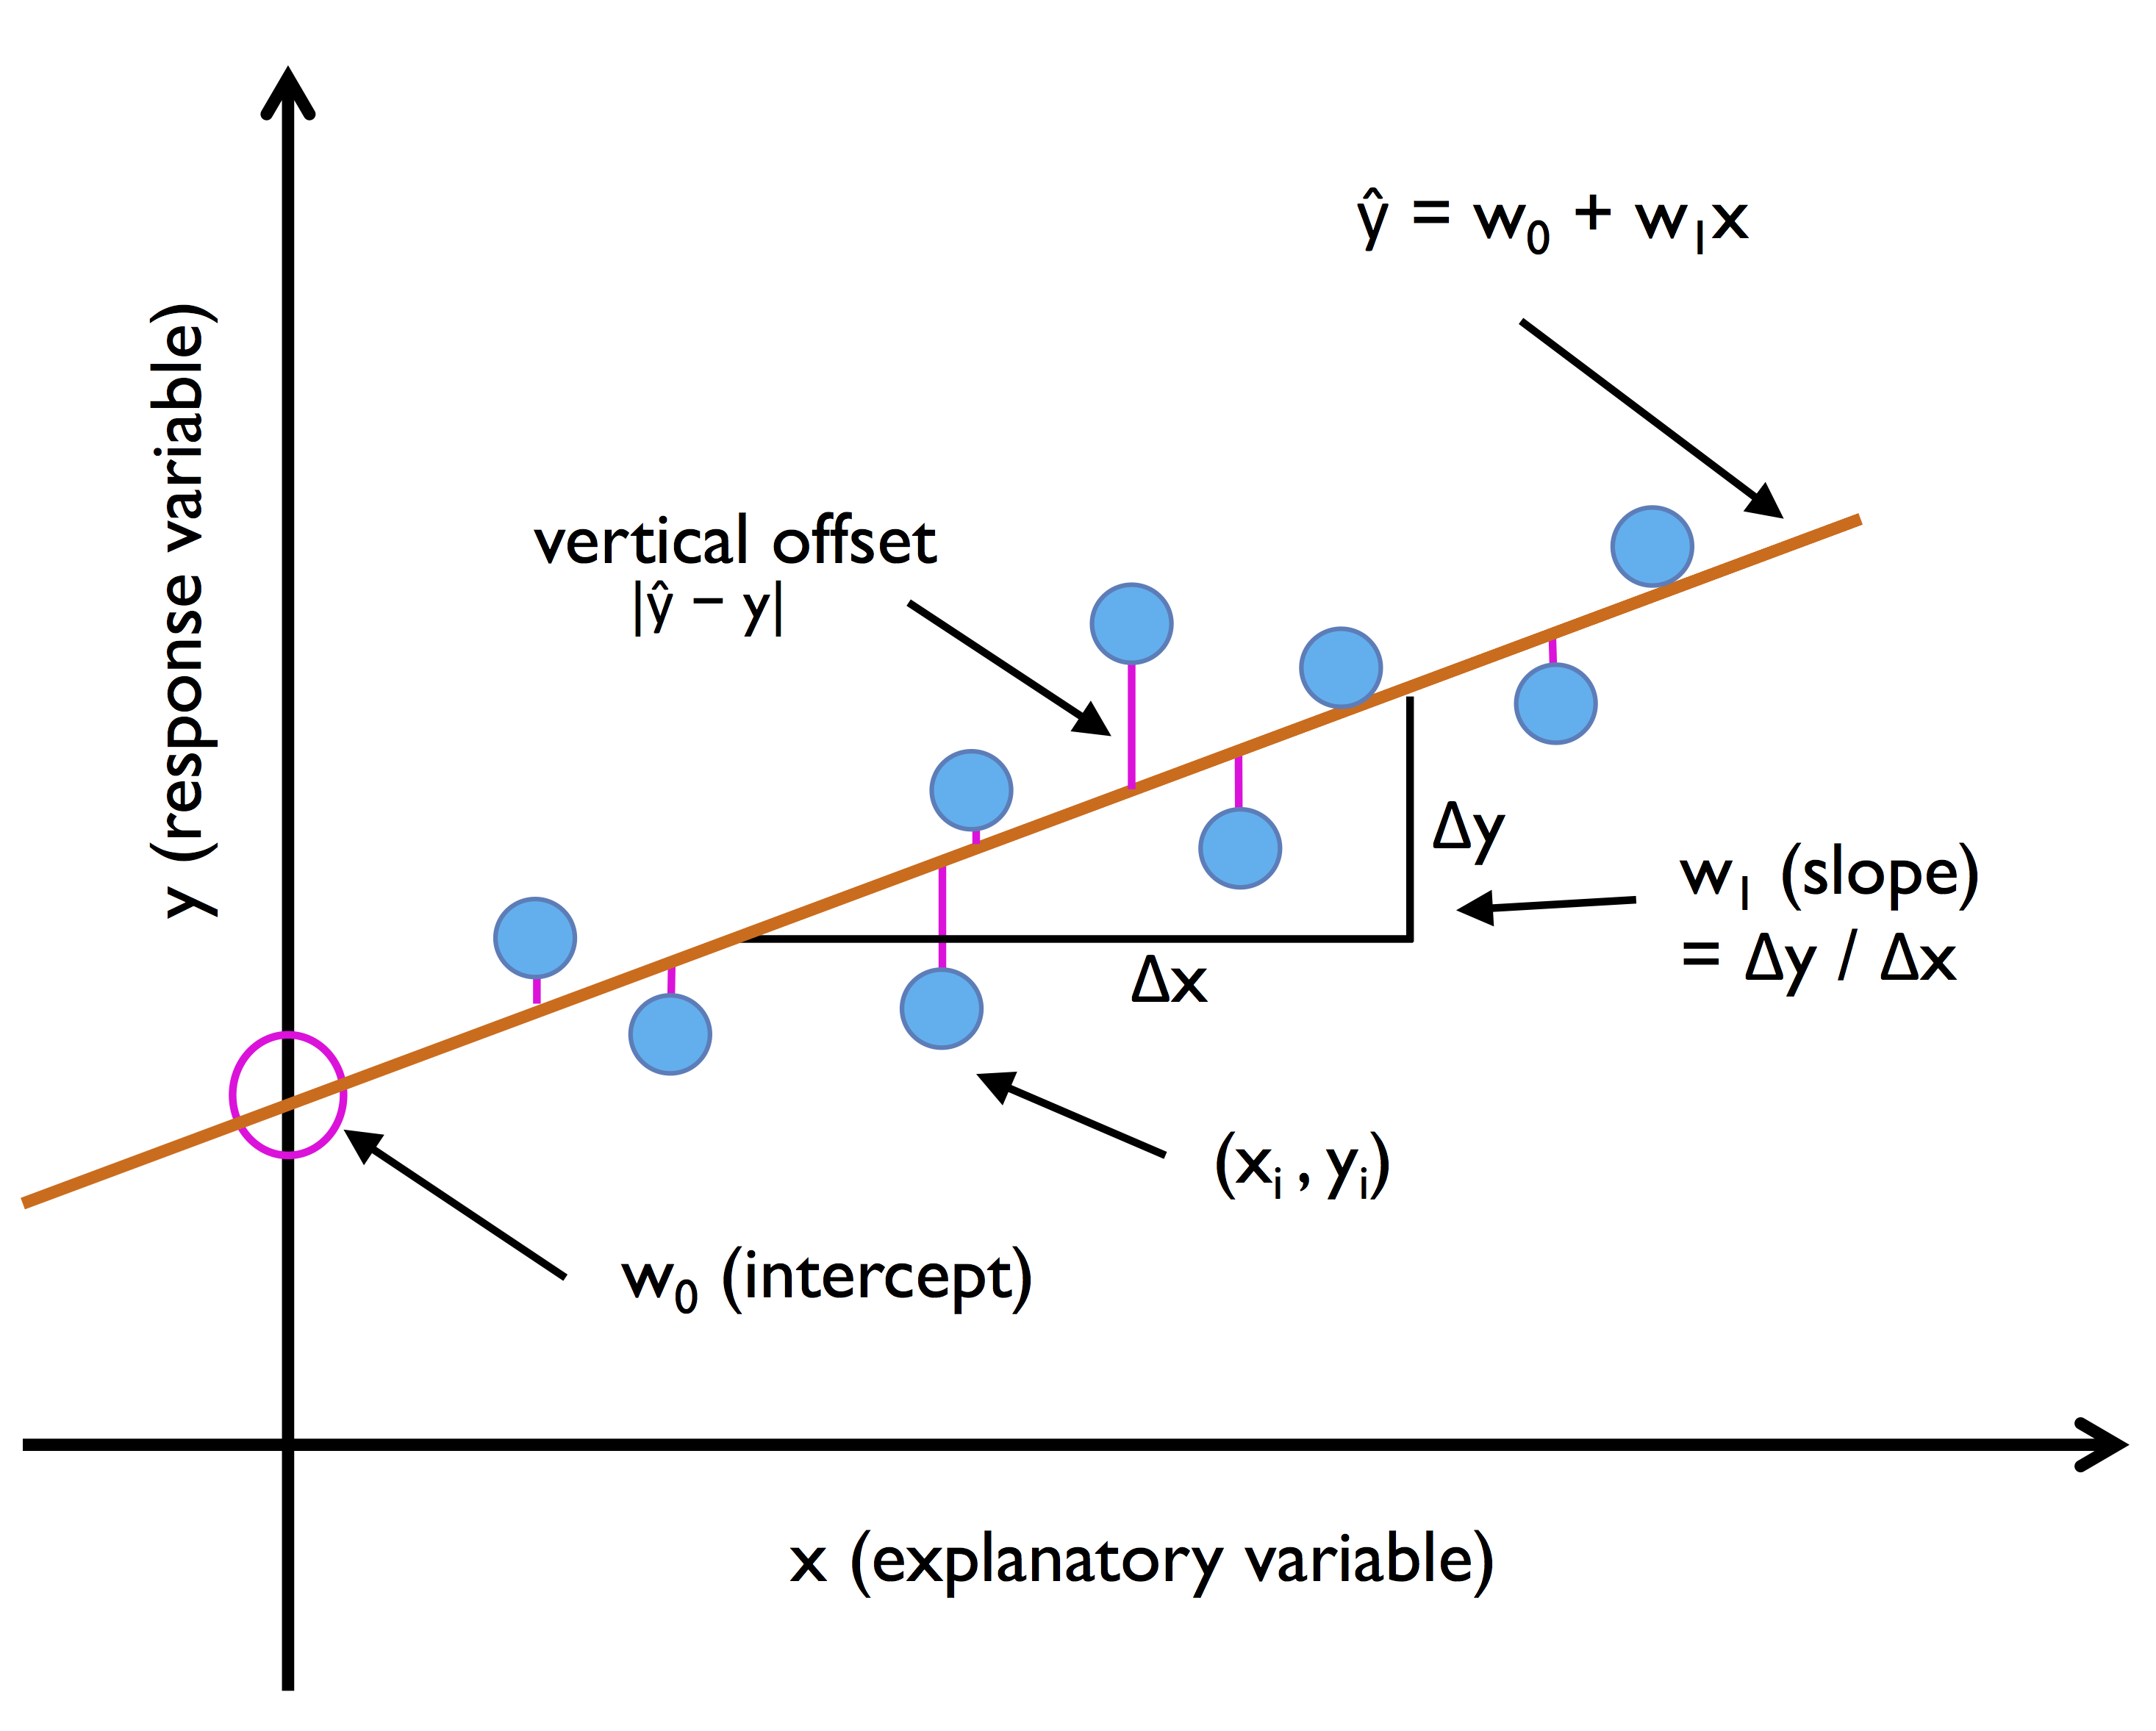
\includegraphics[width=0.63\linewidth]{graphs/fig3.png}
\end{frame}

\begin{frame}{Задача: классификация изображений}
    \begin{figure}
        \begin{subfigure}[b]{\linewidth}
            \centering
            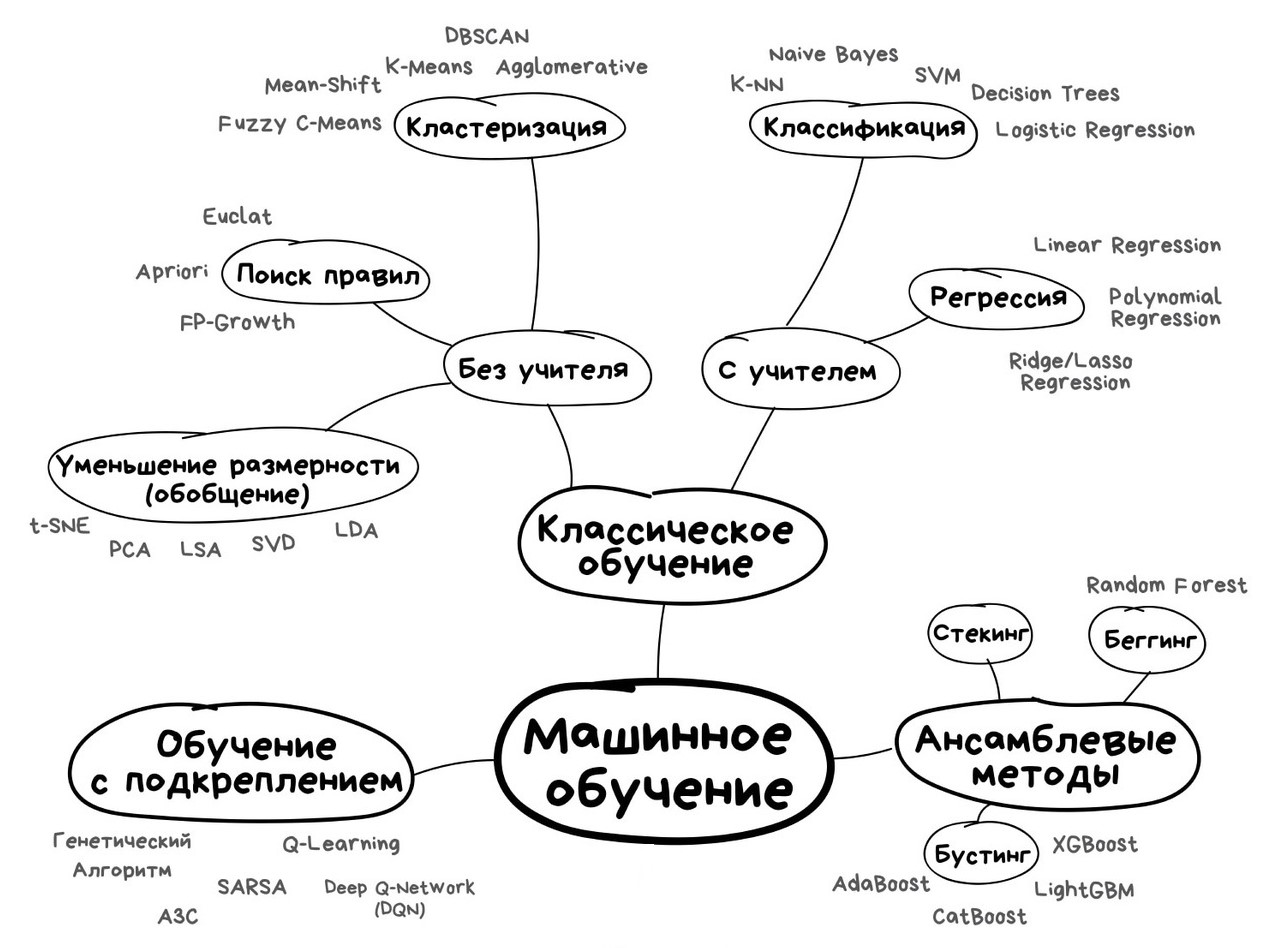
\includegraphics[width=0.385\linewidth]{graphs/fig4.jpg}
        \end{subfigure}
        \pause{}
        \begin{subfigure}[b]{\linewidth}
            \centering
            
\includegraphics[width=0.38\linewidth]{graphs/fig5.jpg}
        \end{subfigure}
    \end{figure}
\end{frame}

\begin{frame}{Задача классификации изображений}
    Постановка задачи:\pause{}
     для заданного изображения найти правильную метку из дискретного набора
    \vfill
    \begin{columns}
        \begin{column}{0.35\linewidth}
            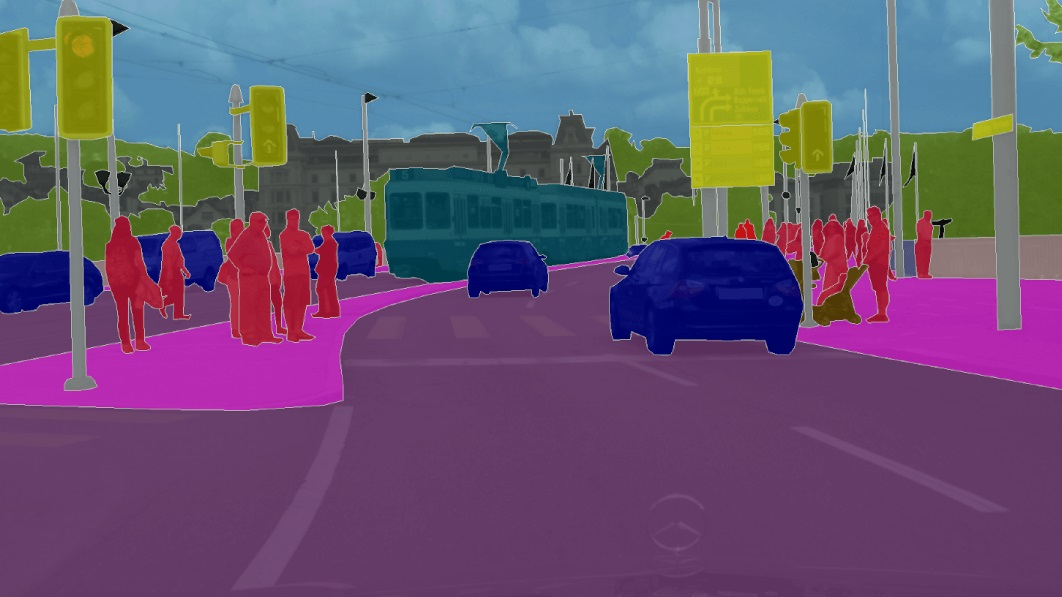
\includegraphics[width=\linewidth]{graphs/fig6.png}
        \end{column}
        \begin{column}{0.65\linewidth}
            \( \{dog, cat, parrot, human, car, \ldots \} \) \\
            \hfill
            \vfill
            \( \Longrightarrow \quad \) cat
        \end{column}
    \end{columns}
\end{frame}

\begin{frame}{Задача классификации изображений}
    Математическая постановка задачи:\pause{} построить функцию
     \( f(x) \rightarrow l\), где \(x\) --- входное изображение,
     \(l\) --- метка из набора
    \pause{}
    \vfill
    \begin{columns}
        \begin{column}{0.49\linewidth}
            \begin{figure}
                \centering
                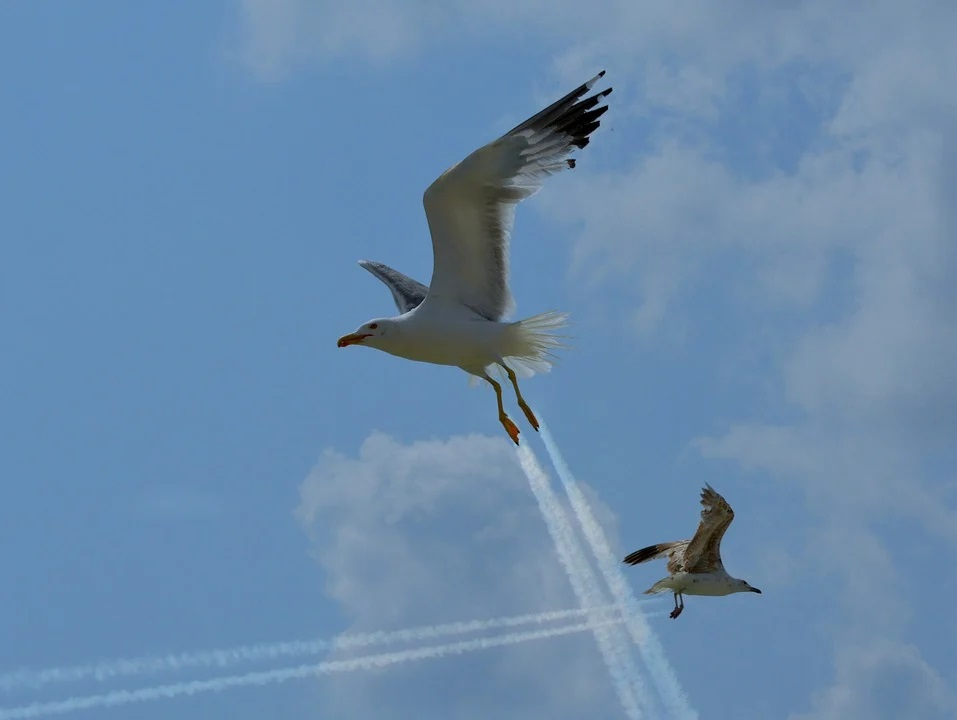
\includegraphics[width=0.85\linewidth]{graphs/fig7.png}
                \caption{Функция сортировки}
            \end{figure}
        \end{column}
        \pause{}
        \begin{column}{0.49\linewidth}
            \begin{figure}
                \centering
                
\includegraphics[width=0.85\linewidth]{graphs/fig8.png}
                \caption{Функция классификации}
            \end{figure}
        \end{column}
    \end{columns}
\end{frame}

\begin{frame}{Семантический разрыв (semantic gap)}
    \begin{columns}
        \begin{column}{0.4\linewidth}
            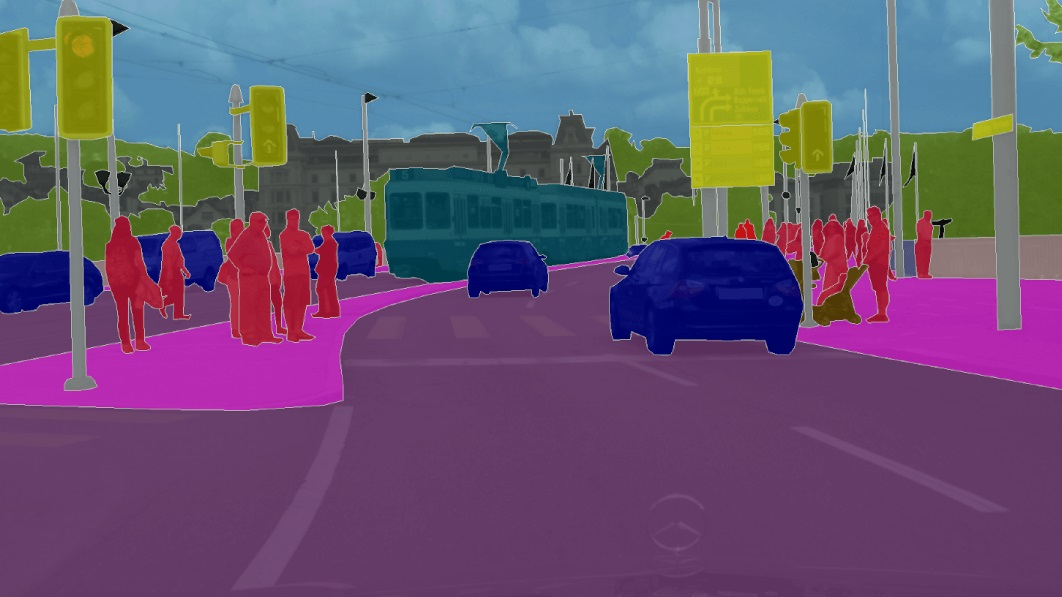
\includegraphics[width=\linewidth]{graphs/fig6.png}
        \end{column}
        \pause{}
        \begin{column}{0.6\linewidth}
            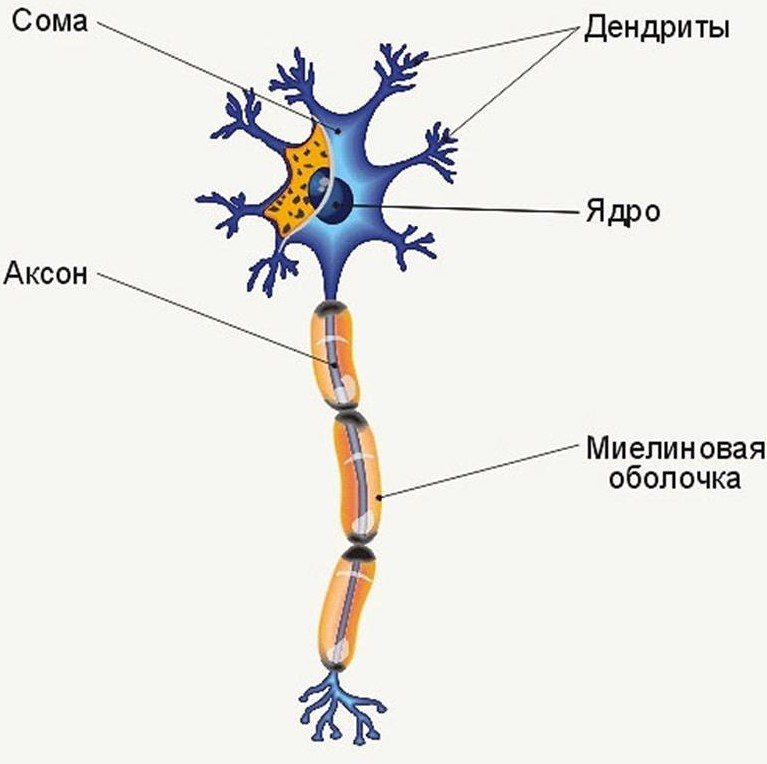
\includegraphics[width=\linewidth]{graphs/fig9.png}
        \end{column}
    \end{columns}
\end{frame}

\begin{frame}{Сложности: смена ракурса}
    \begin{figure}
        \begin{subfigure}[b]{0.32\linewidth}
            \centering
            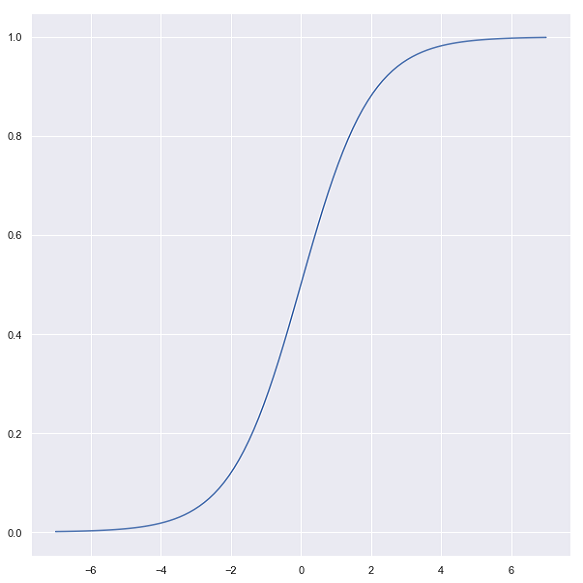
\includegraphics[width=\linewidth]{graphs/fig11.png}
        \end{subfigure}
        \begin{subfigure}[b]{0.32\linewidth}
            \centering
            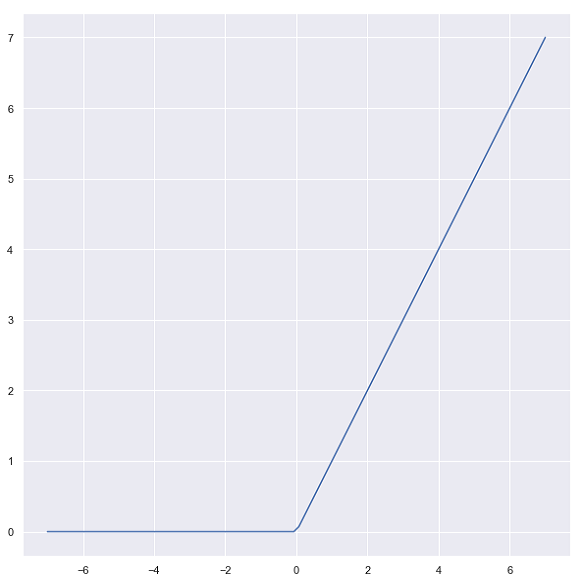
\includegraphics[width=\linewidth]{graphs/fig12.png}
        \end{subfigure}
        \begin{subfigure}[b]{0.32\linewidth}
            \centering
            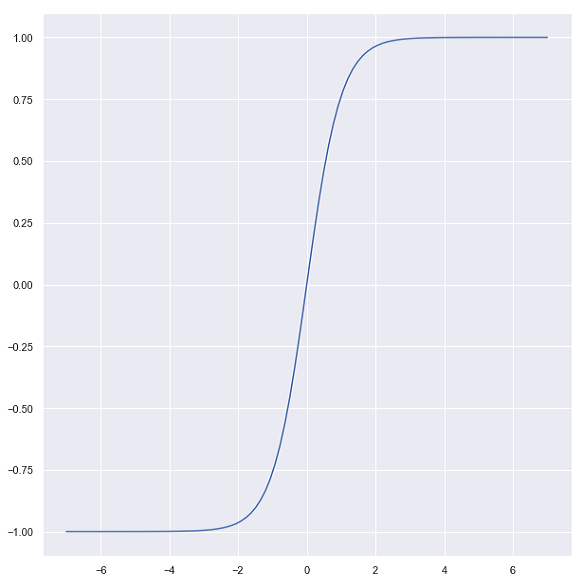
\includegraphics[width=\linewidth]{graphs/fig13.png}
        \end{subfigure}
    \end{figure}
\end{frame}

\begin{frame}{Сложности: разное освещение}
    \begin{figure}
        \begin{subfigure}[b]{0.3\linewidth}
            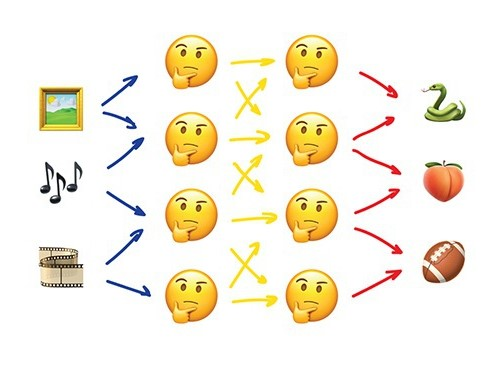
\includegraphics[width=\linewidth]{graphs/fig14.jpg}
        \end{subfigure}
        \begin{subfigure}[b]{0.3\linewidth}
            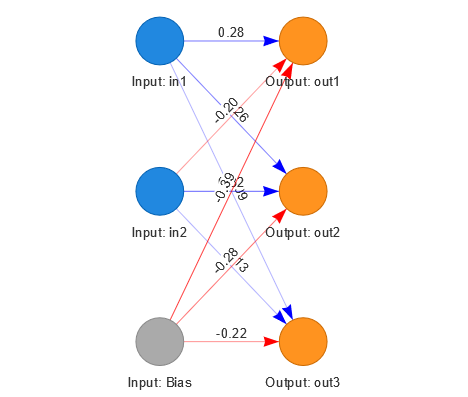
\includegraphics[width=\linewidth]{graphs/fig15.jpg}
        \end{subfigure}
        \begin{subfigure}[b]{0.3\linewidth}
            
\includegraphics[width=\linewidth]{graphs/fig16.jpg}
        \end{subfigure}
    \end{figure}
\end{frame}

\begin{frame}{Сложности: вариация форм (``Cats are liquid'')}
    \begin{figure}
        \begin{subfigure}[b]{0.3\linewidth}
            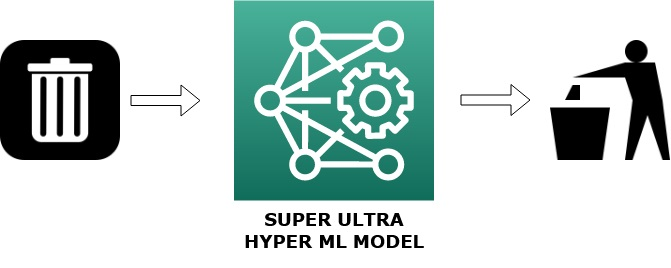
\includegraphics[width=\linewidth]{graphs/fig17.jpg}
        \end{subfigure}
        \begin{subfigure}[b]{0.3\linewidth}
            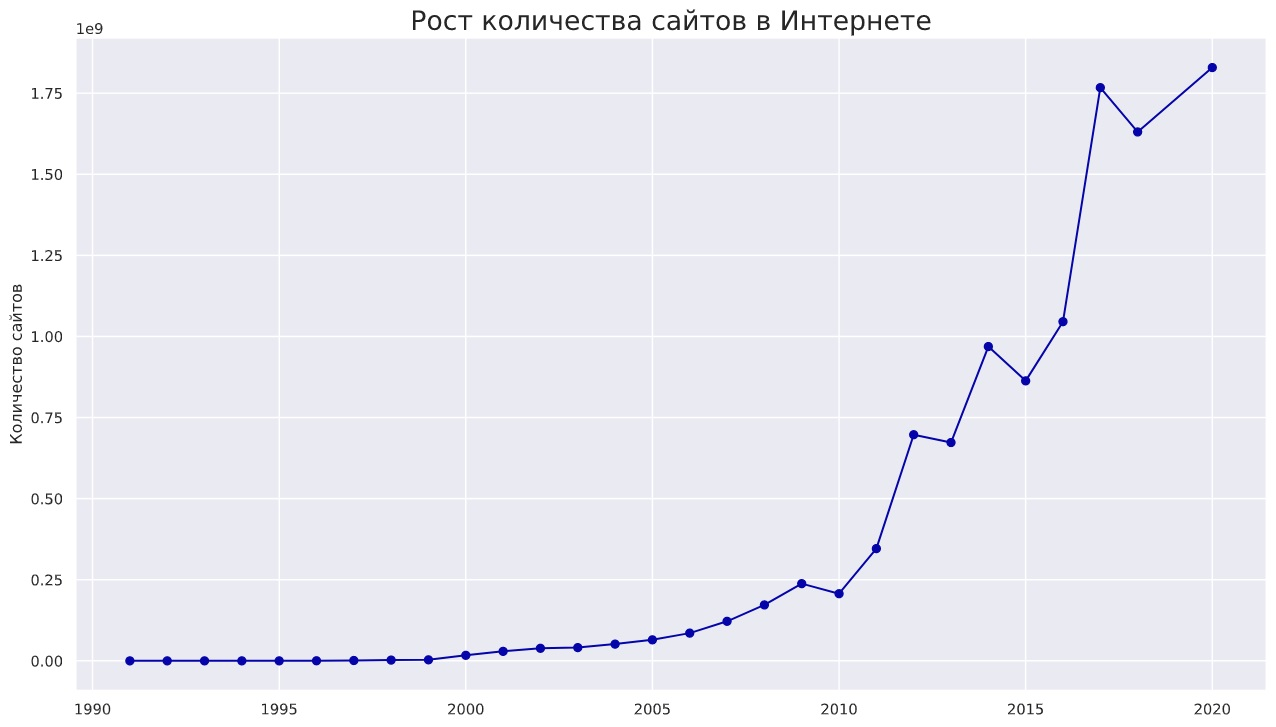
\includegraphics[width=\linewidth]{graphs/fig18.jpg}
        \end{subfigure}
        \begin{subfigure}[b]{0.3\linewidth}
            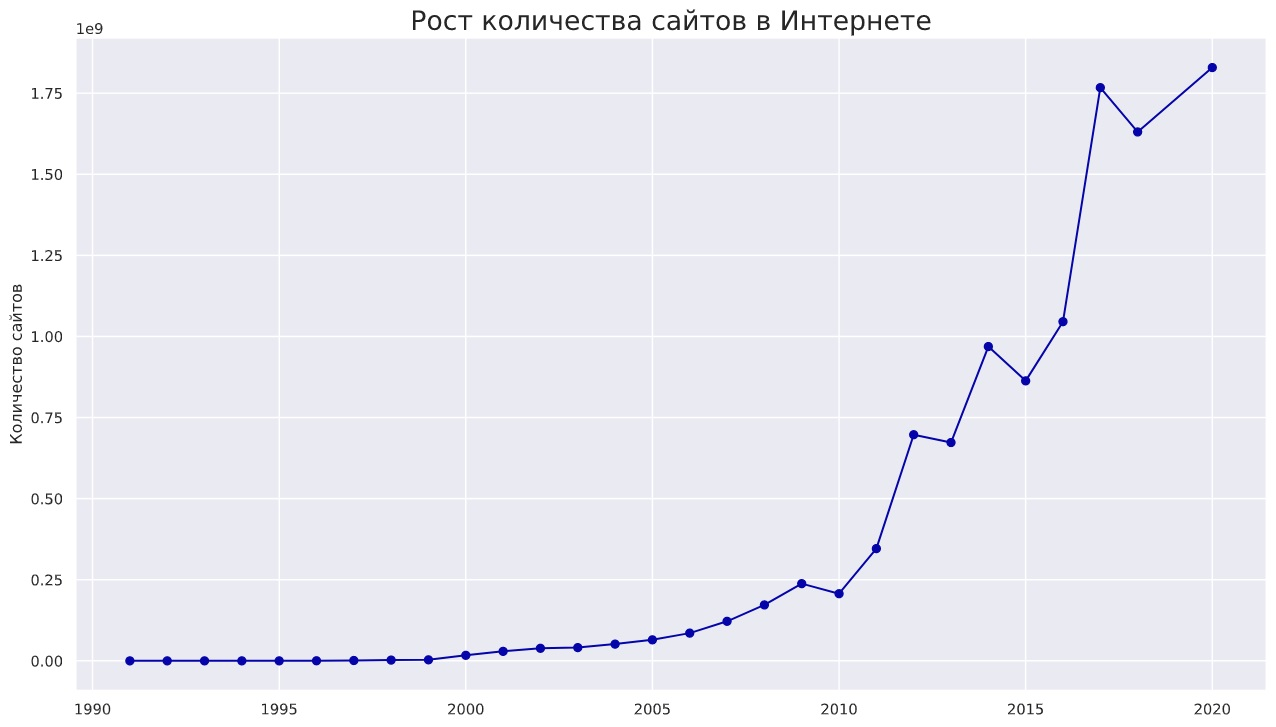
\includegraphics[width=\linewidth]{graphs/fig19.png}
        \end{subfigure}
    \end{figure}
\end{frame}

\begin{frame}{Сложности: внутриклассовая вариативность}
    \begin{figure}
        
\includegraphics[width=0.69\linewidth]{graphs/fig20.jpg}
    \end{figure}
\end{frame}

\begin{frame}{Задача классификации изображений}
    \begin{center}
        
\includegraphics[width=0.68\linewidth]{graphs/fig8.png}
    \end{center}
    Таким образом, \textbf{очевидный} способ запрограммировать эту функцию не
     был найден
\end{frame}

\begin{frame}{Задача классификации изображений}
    Конечно, было предпринято множество попыток, например
    \vfill
    \begin{columns}
        \begin{column}{0.27\linewidth}
            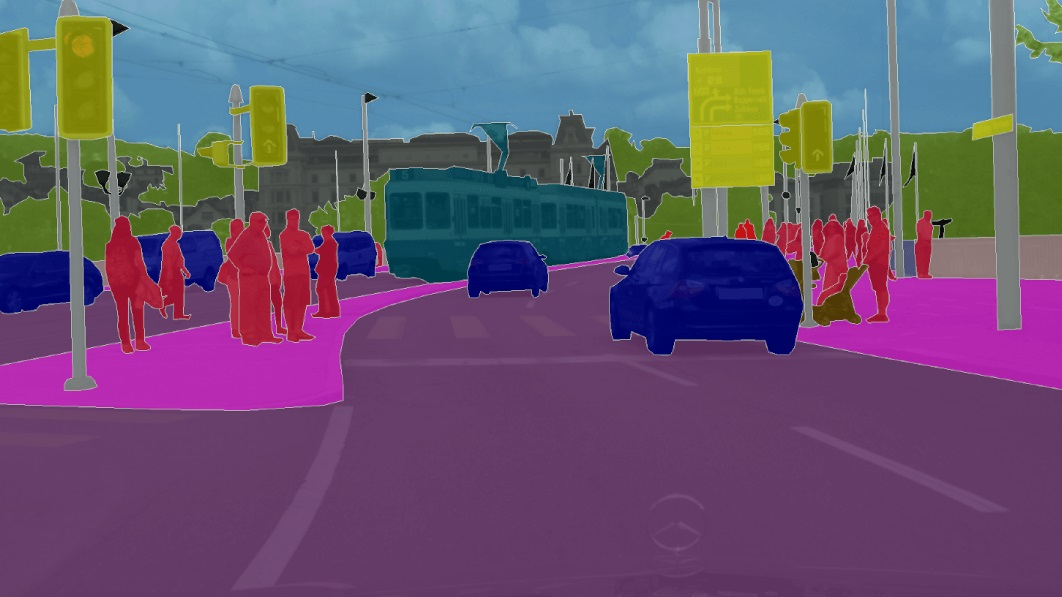
\includegraphics[width=\linewidth]{graphs/fig6.png}
        \end{column}
        \pause{}
        \begin{column}{0.1\linewidth}
            \centering
            \( \longrightarrow \) \\
            поиск границ
        \end{column}
        \begin{column}{0.27\linewidth}
            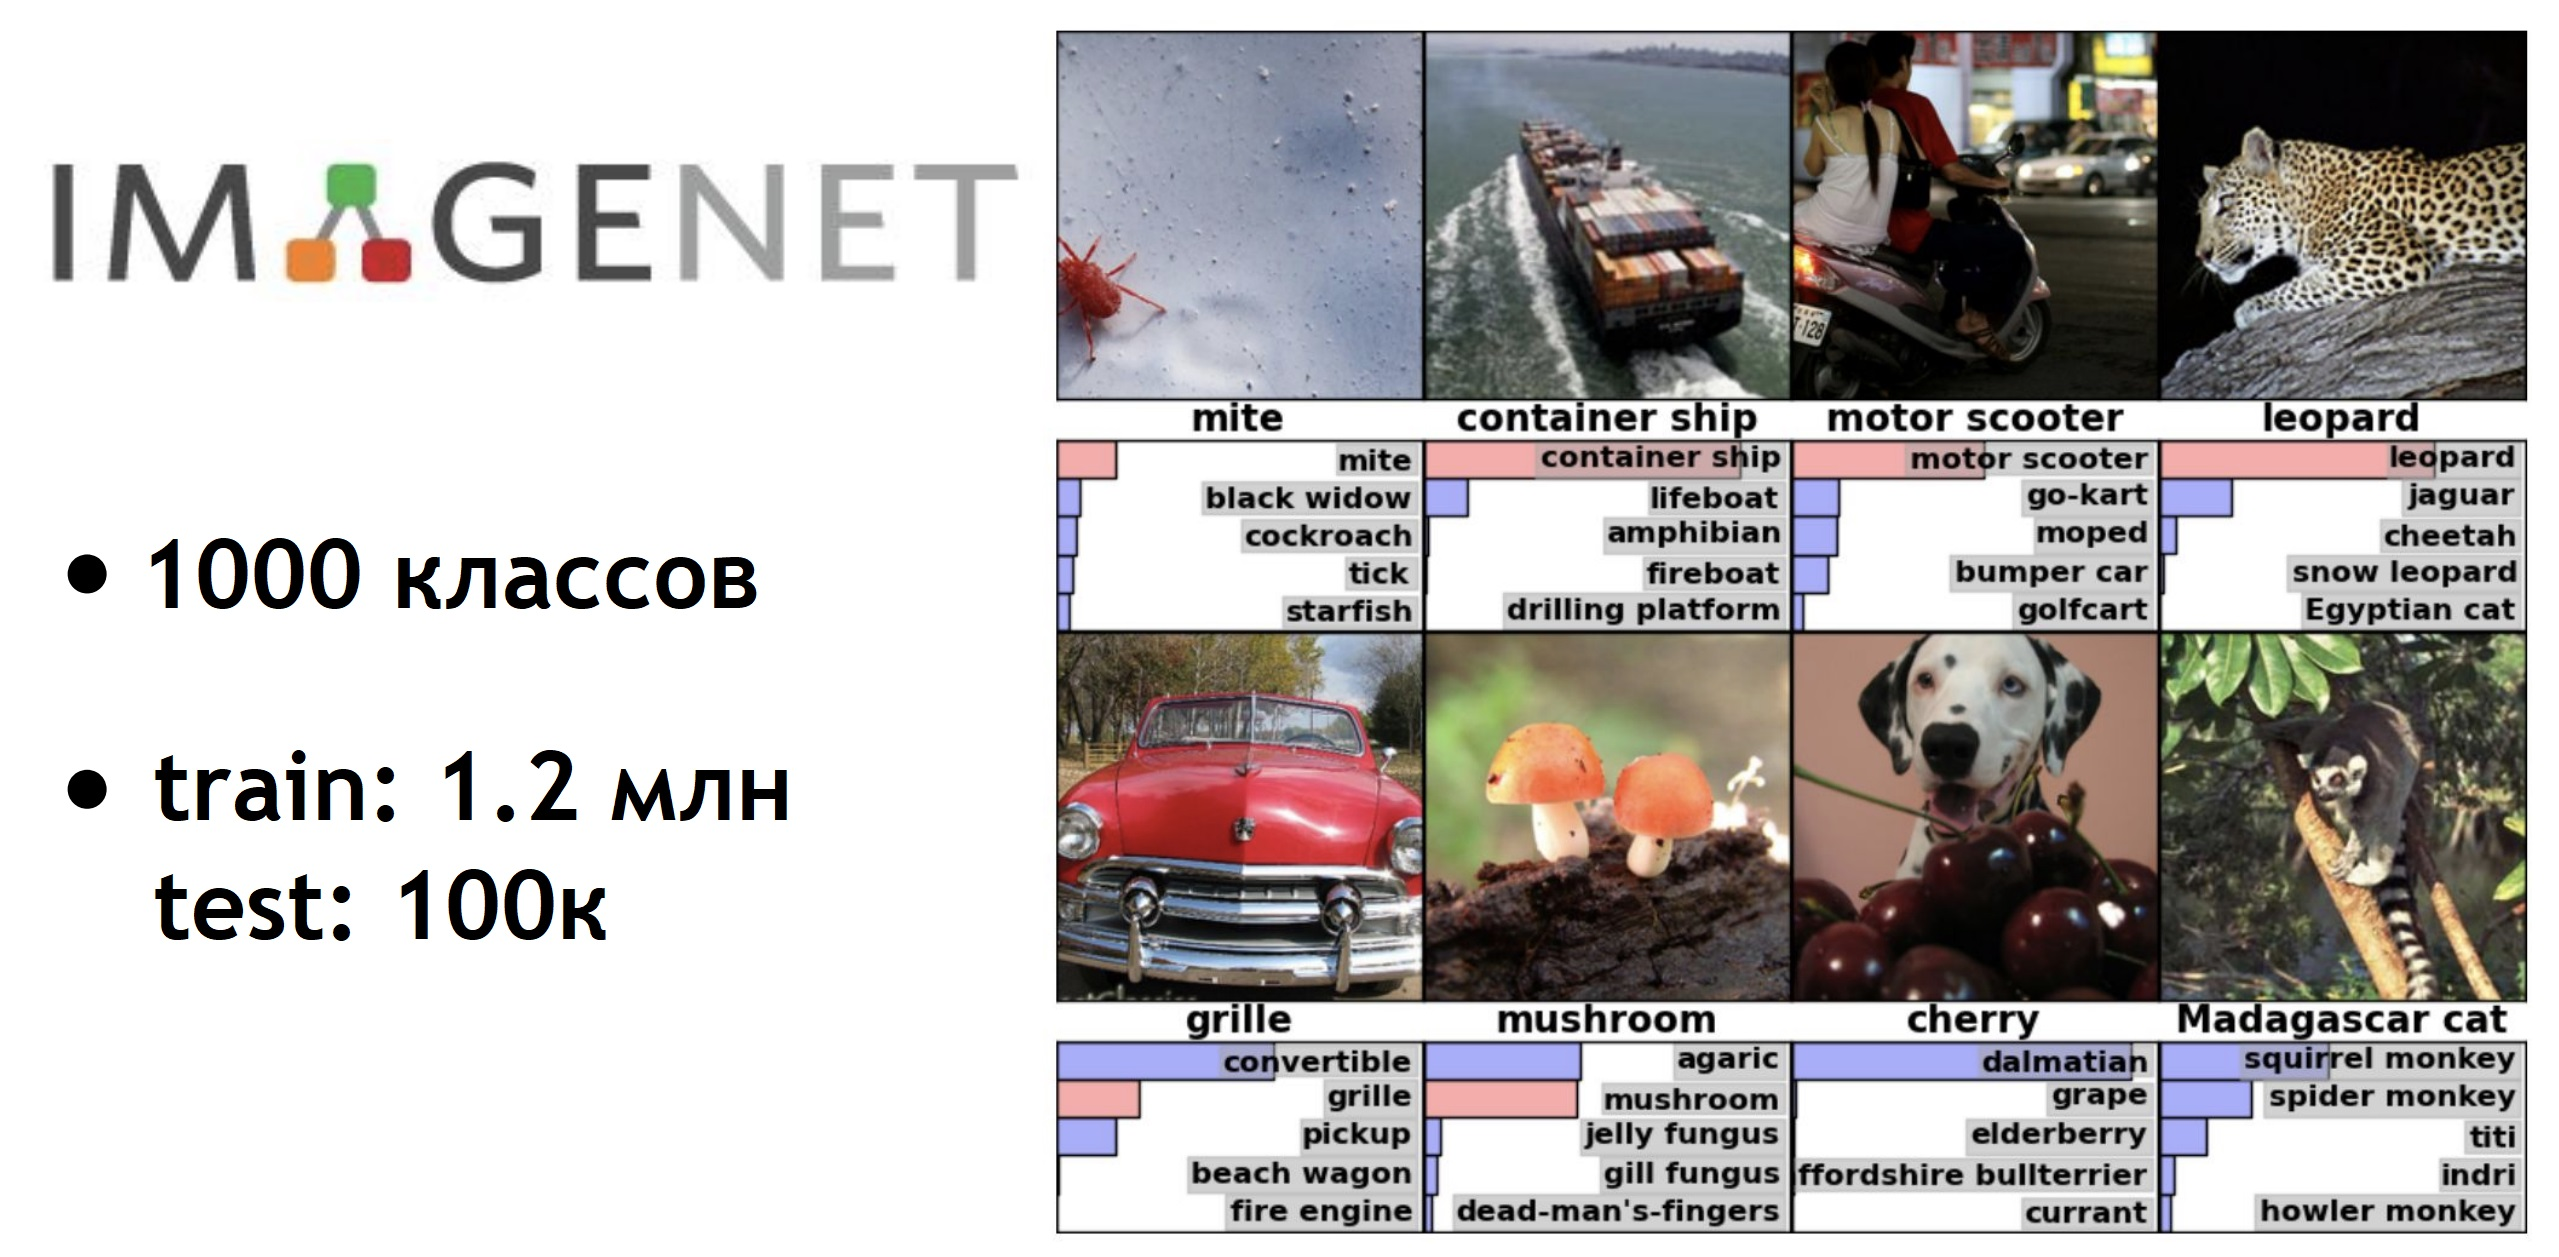
\includegraphics[width=\linewidth]{graphs/fig21.png}
        \end{column}
        \pause{}
        \begin{column}{0.1\linewidth}
            \centering
            \( \longrightarrow \) \\
            поиск углов
        \end{column}
        \begin{column}{0.1\linewidth}
            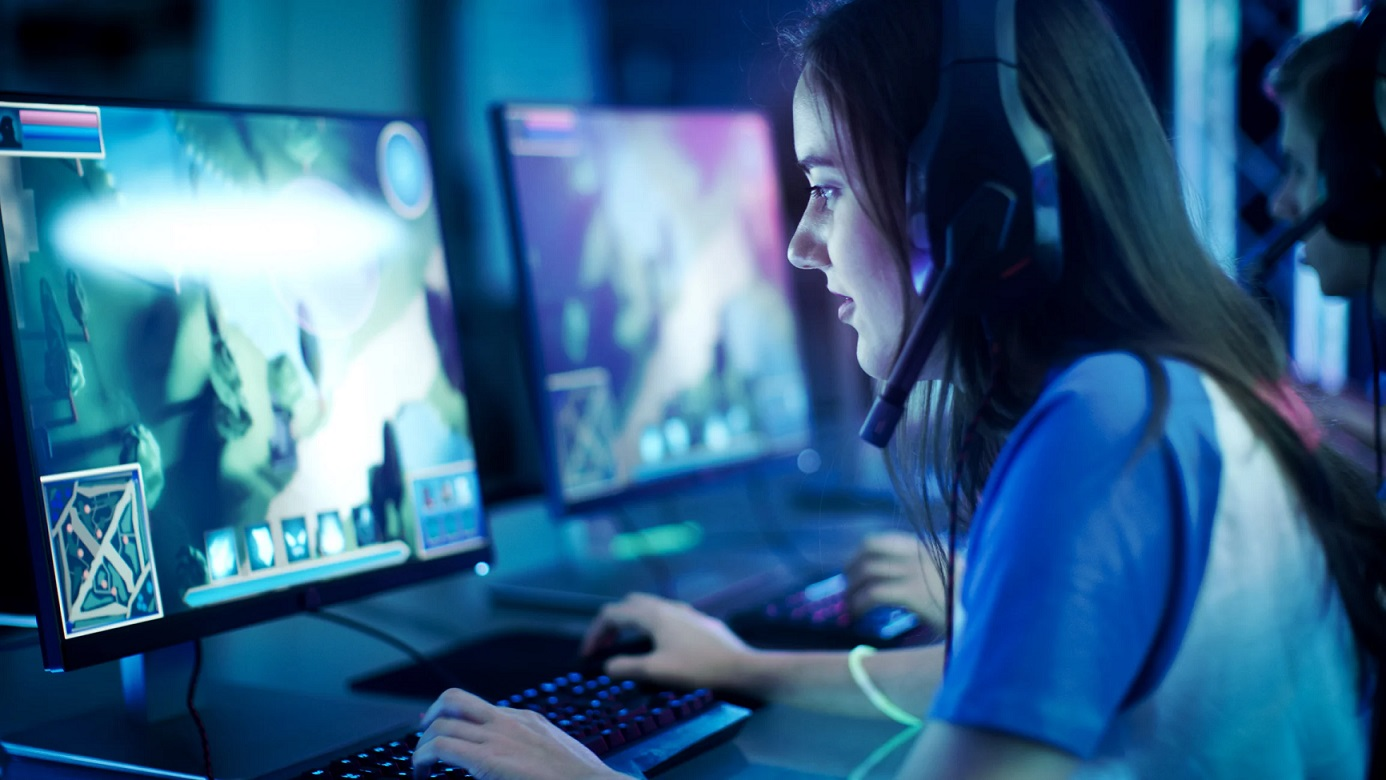
\includegraphics[width=\linewidth]{graphs/fig22.png}
        \end{column}
        \pause{}
        \begin{column}{0.05\linewidth}
            \centering
            \( \longrightarrow  \) \\
            \( ? \)
        \end{column}
    \end{columns}
\end{frame}

\begin{frame}{Машинное обучение: подход от данных}
    \pause{}
    \centering
    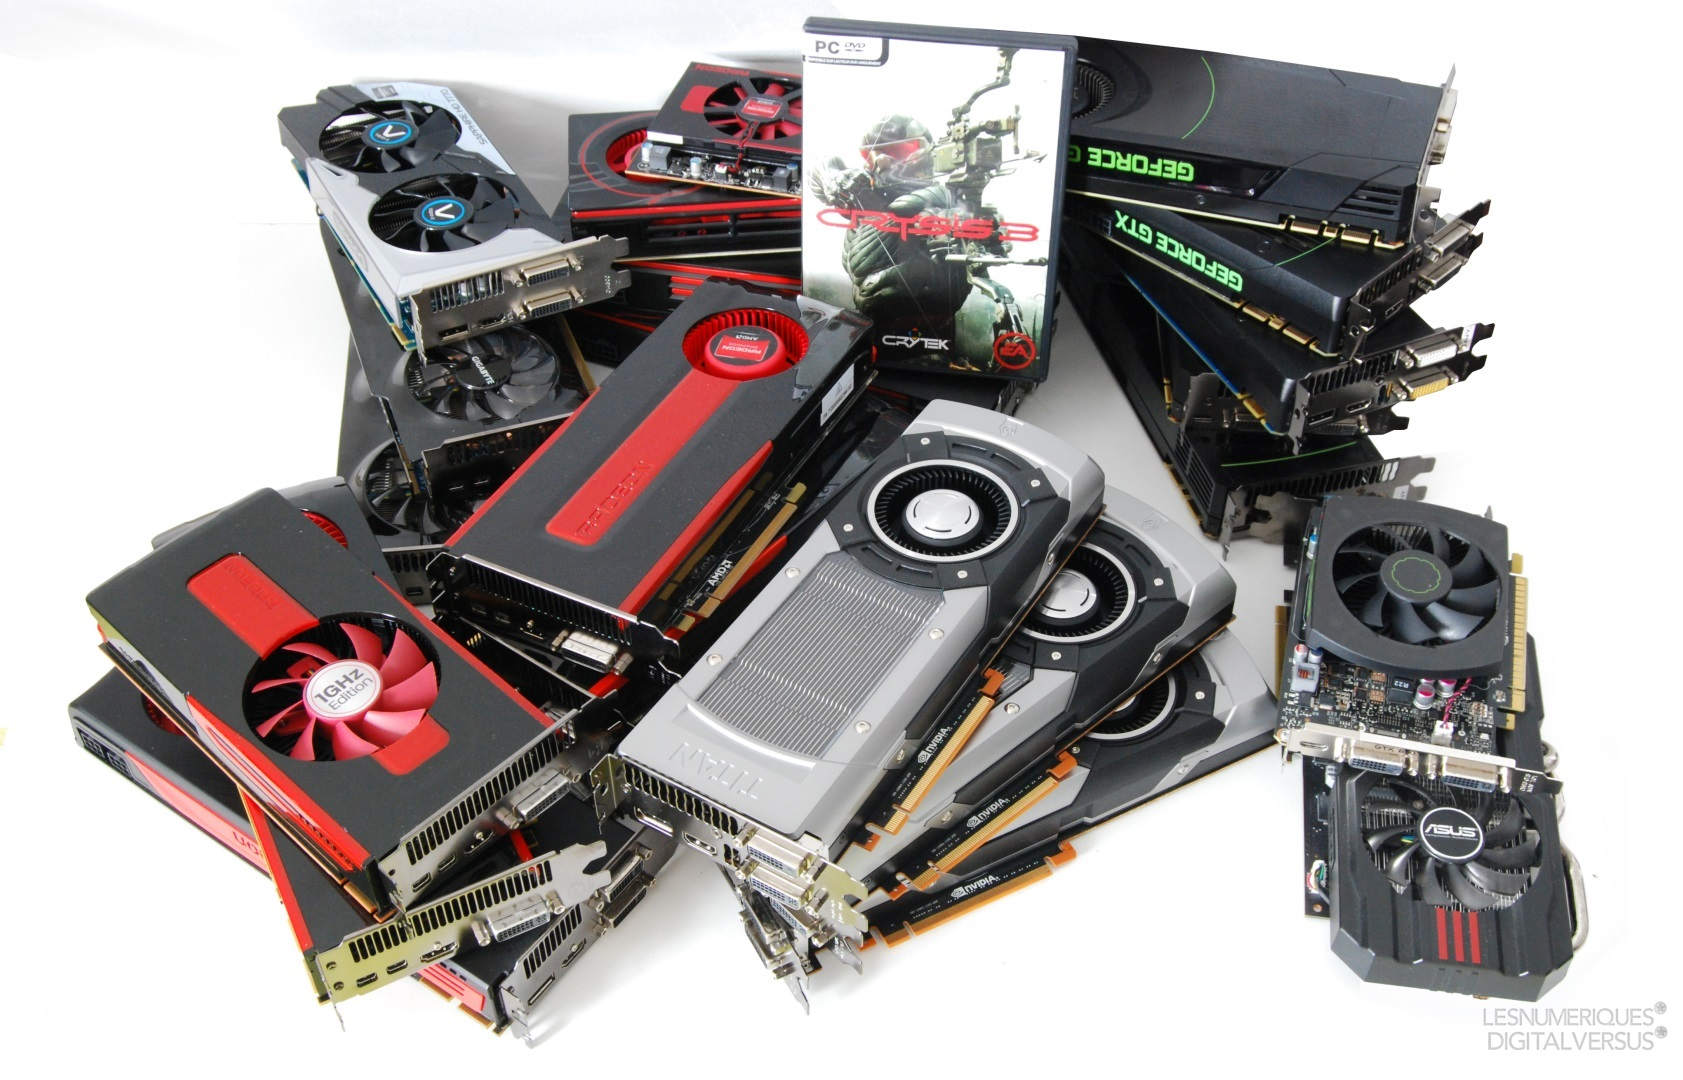
\includegraphics[width=0.715\linewidth]{graphs/fig23.jpg}
\end{frame}

\begin{frame}{Машинное обучение: подход от данных}
    \begin{itemize}
        \item Алгоритмы \textbf{машинного обучения} (machine learning, ML) ---
         класс алгоритмов, которые \textbf{не программируются явно}, но
         \textbf{подстраиваются под загруженные данные}
        \pause{}
        \item \textbf{Обучающая выборка} --- набор примеров с правильными
         ответами
    \end{itemize}
    \pause{}
    \begin{figure}
        \begin{subfigure}[b]{0.1\linewidth}
            \includegraphics[width=\linewidth]{graphs/fig46.jpg}
            \subcaption*{`cat'}
        \end{subfigure}
        \begin{subfigure}[b]{0.1\linewidth}
            
\includegraphics[width=\linewidth]{graphs/fig24.jpg}
            \subcaption*{`dog'}
        \end{subfigure}
        \begin{subfigure}[b]{0.1\linewidth}
            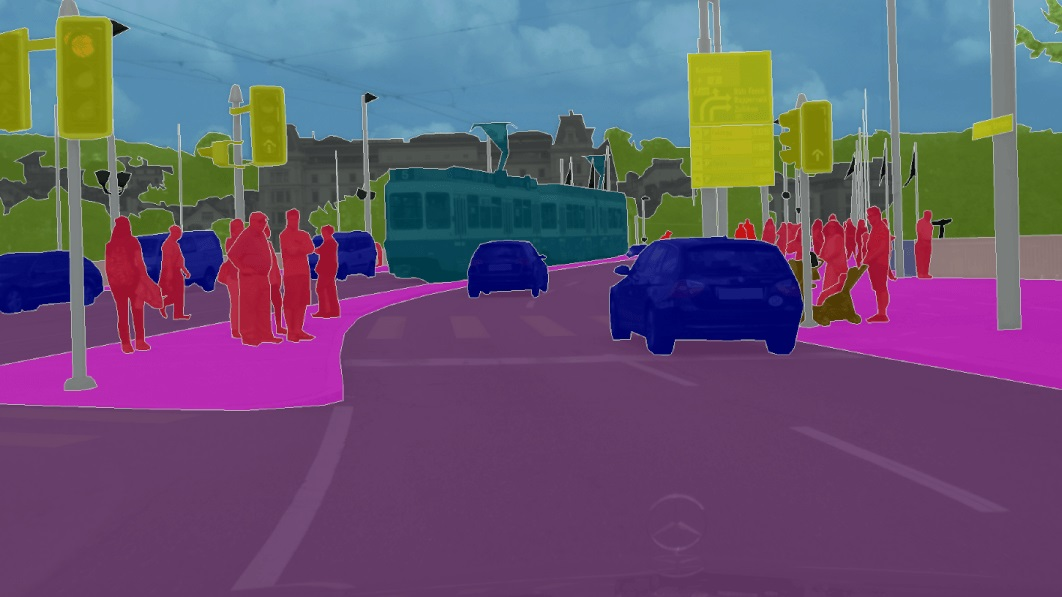
\includegraphics[width=\linewidth]{graphs/fig33.jpg}
            \subcaption*{`ninja'}
        \end{subfigure}
        \begin{subfigure}[b]{0.1\linewidth}
            \includegraphics[width=\linewidth]{graphs/fig47.png}
            \subcaption*{`cat'}
        \end{subfigure}
        \begin{subfigure}[b]{0.1\linewidth}
            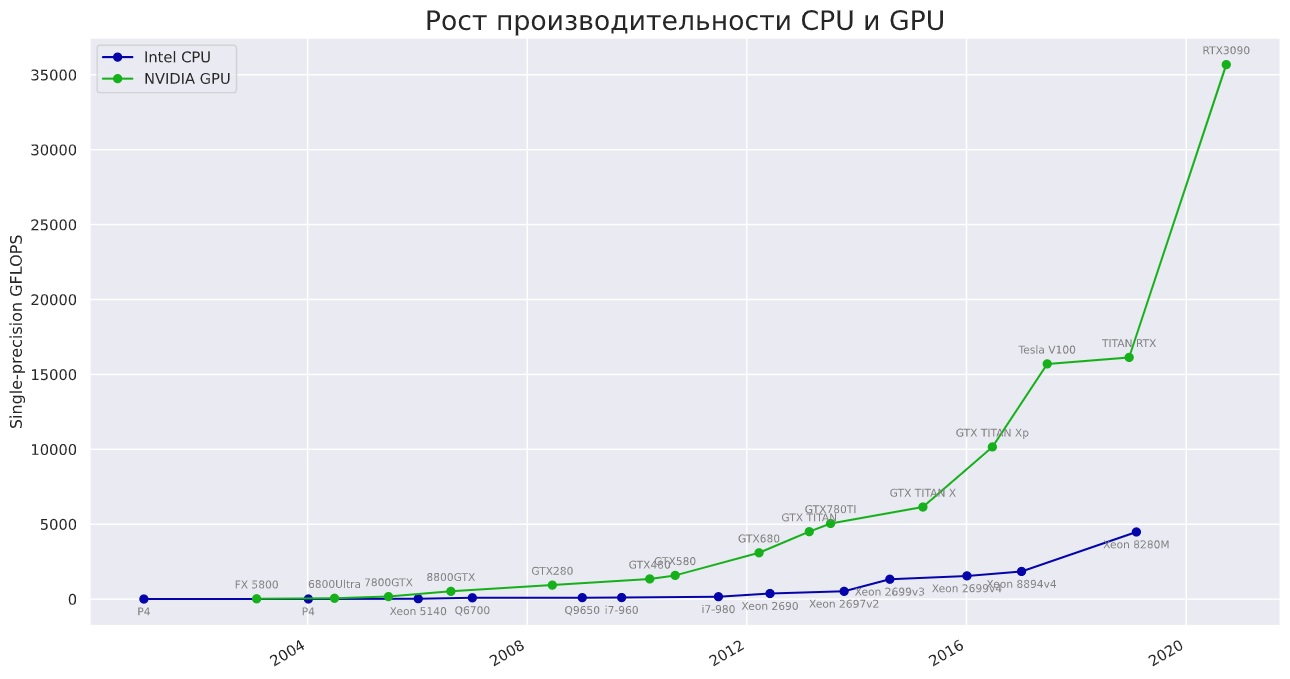
\includegraphics[width=\linewidth]{graphs/fig25.jpg}
            \subcaption*{`dog'}
        \end{subfigure}
        \begin{subfigure}[b]{0.1\linewidth}
            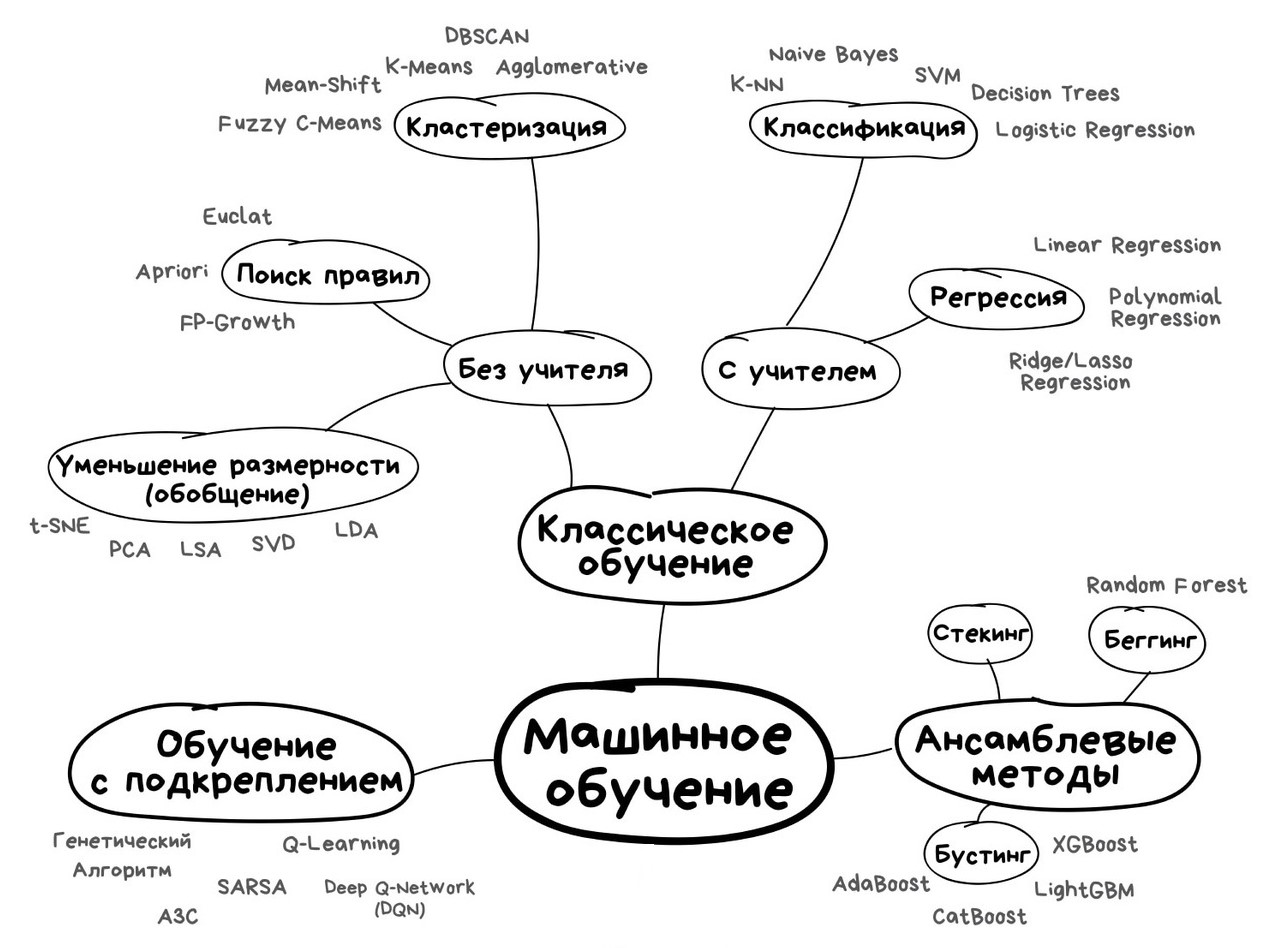
\includegraphics[width=\linewidth]{graphs/fig31.jpg}
            \subcaption*{`cat'}
        \end{subfigure}
        \begin{subfigure}[b]{0.1\linewidth}
            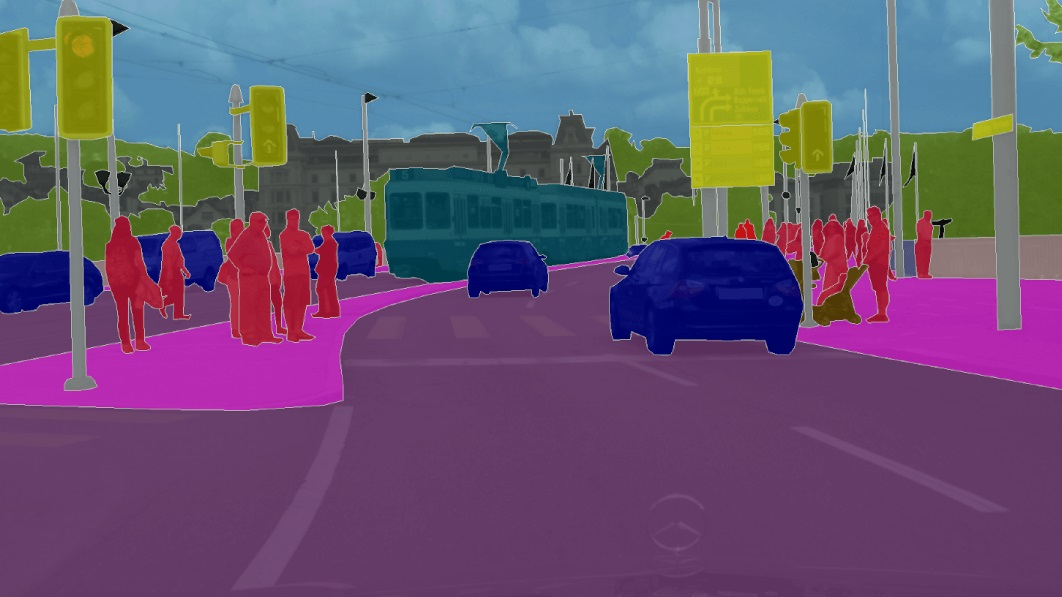
\includegraphics[width=\linewidth]{graphs/fig32.jpg}
            \subcaption*{`ninja'}
        \end{subfigure}
        \begin{subfigure}[b]{0.1\linewidth}
            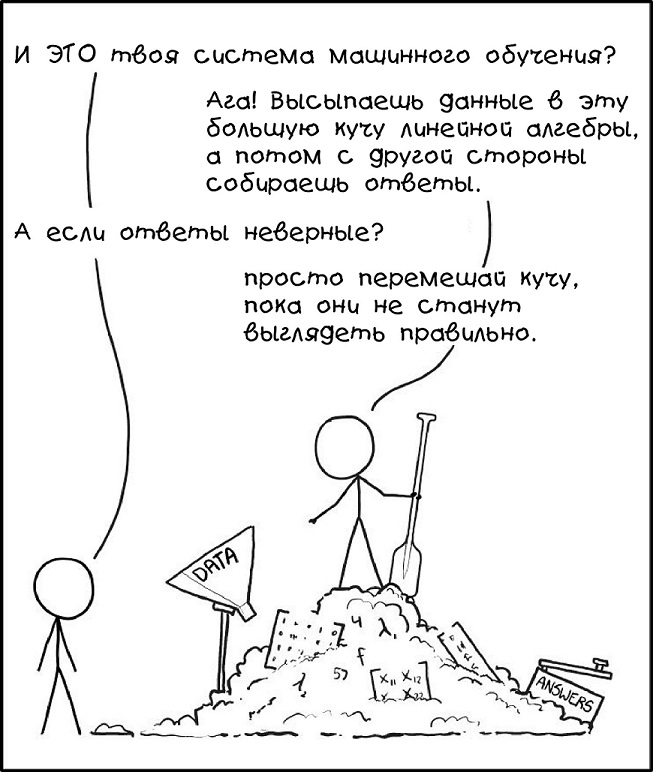
\includegraphics[width=\linewidth]{graphs/fig34.jpg}
            \subcaption*{`dog'}
        \end{subfigure}
        \begin{subfigure}[b]{0.1\linewidth}
            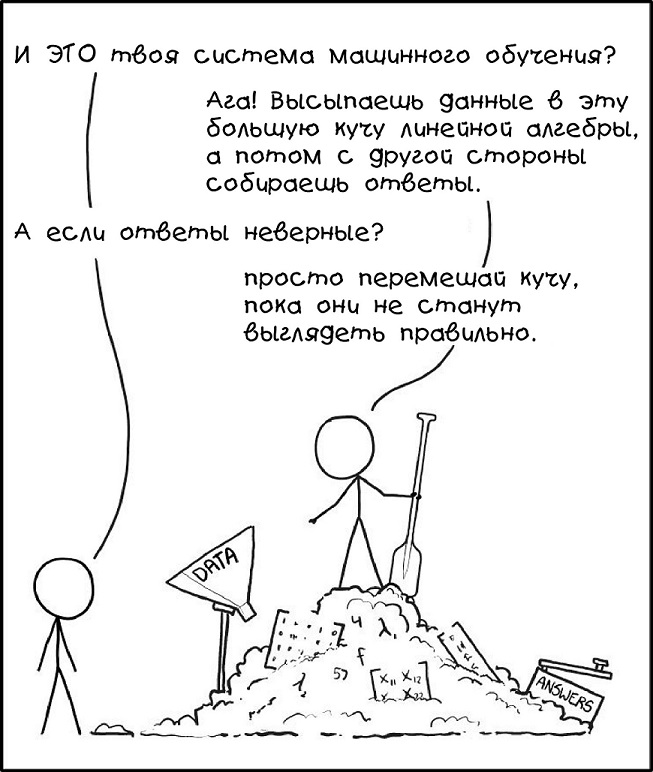
\includegraphics[width=\linewidth]{graphs/fig35.jpg}
            \subcaption*{`cat'}
        \end{subfigure}
        \caption{Пример обучающей выборки}
    \end{figure}
\end{frame}

\begin{frame}{Машинное обучение: подход от данных}
    Машинное обучение появляется когда:
    \begin{itemize}
        \item мы не можем создать точный алгоритм решения задачи, потому что
         слишком мало понимаем лежащие в её основах процессы и
          \textbf{не можем построить} точную модель этих процессов (в отличии,
           скажем, от моделей в физике)
         \pause{}
         \item но можем собрать \textbf{большое} количество данных с примерами
          правильного решения задачи (обучающую выборку)! 
    \end{itemize}
    \pause{}
    Методы машинного обучения пытаются \textbf{восстанавливать модели} на
     основе \textbf{данных}, а не исходя из понимания природы.
\end{frame}

\begin{frame}{Машинное обучение: подход от данных}
    Таким образом, наша функция
    \begin{center}
        
\includegraphics[width=0.25\linewidth]{graphs/fig8.png}
    \end{center}
    \pause{}
    превращается в две:
    \hfill
    \begin{columns}
        \begin{column}{0.4\linewidth}
            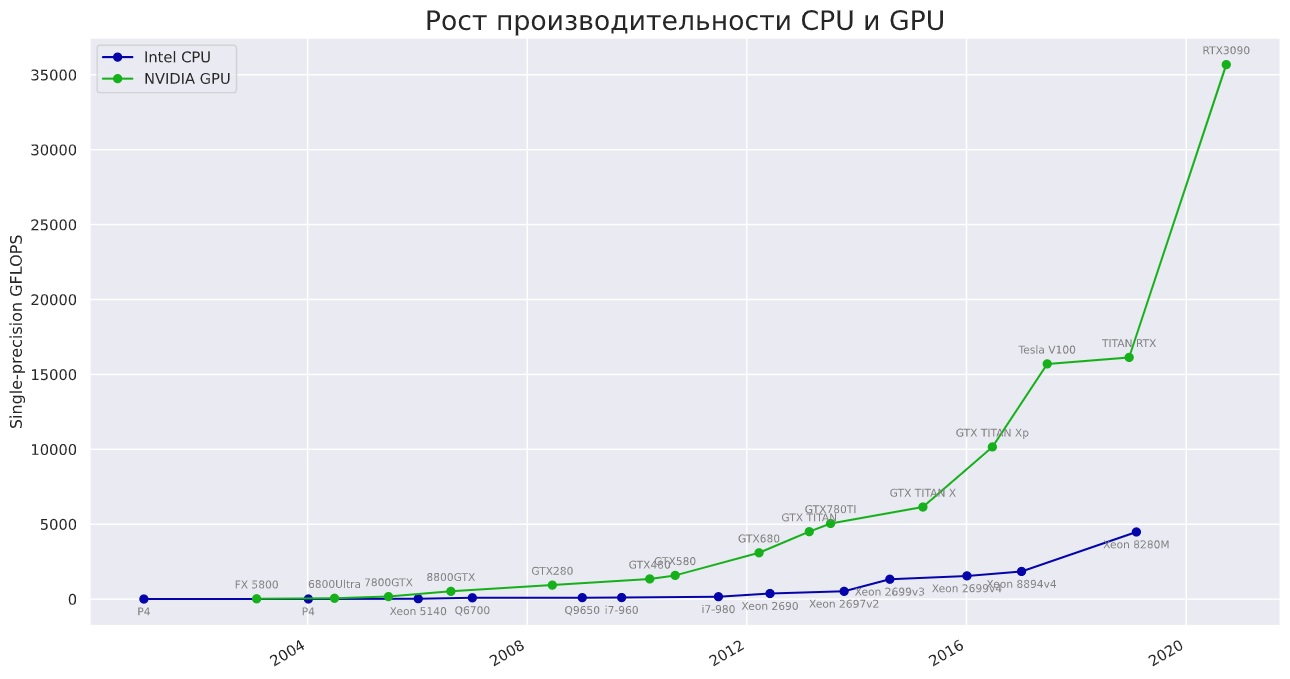
\includegraphics[width=\linewidth]{graphs/fig26.png}
        \end{column}
        \begin{column}{0.4\linewidth}
            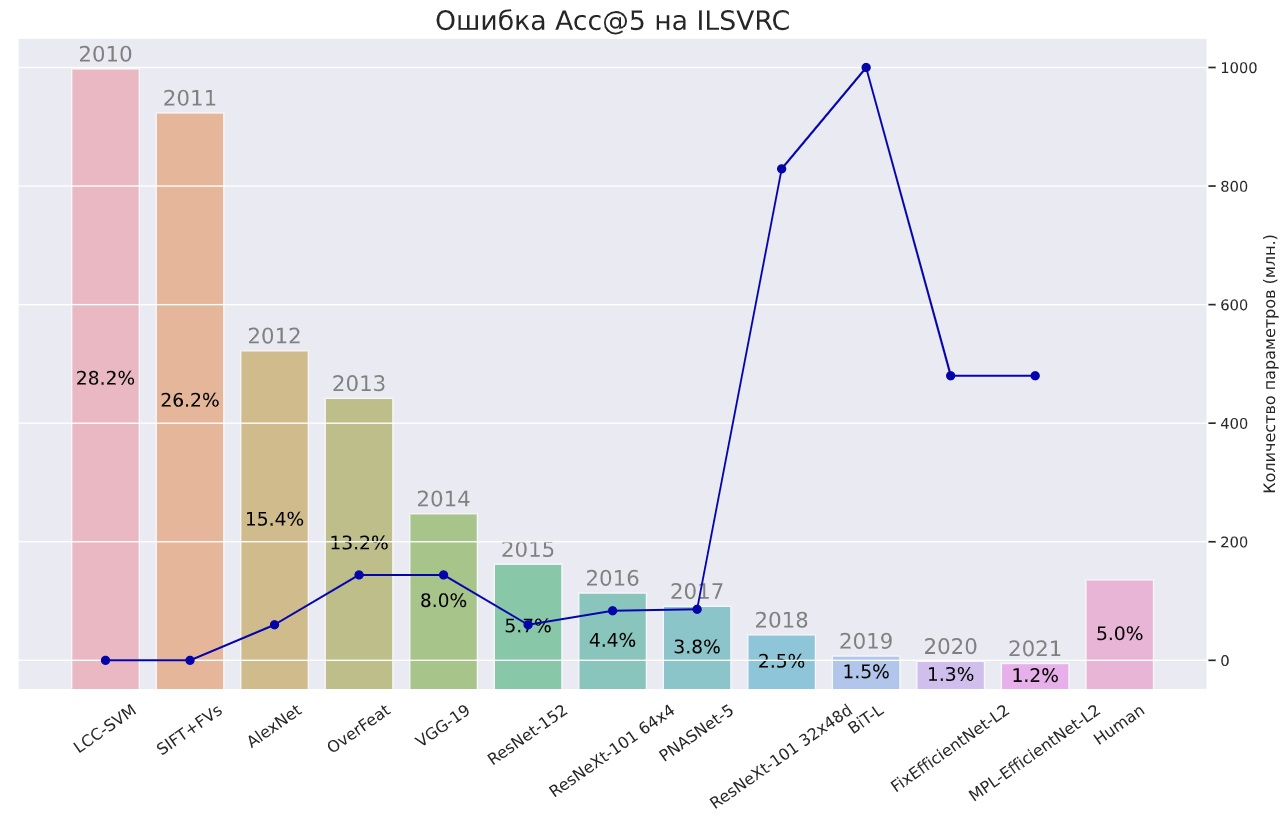
\includegraphics[width=\linewidth]{graphs/fig27.png}
        \end{column}
    \end{columns}
\end{frame}

\begin{frame}{Две ``зимы искусственного интеллекта''}
    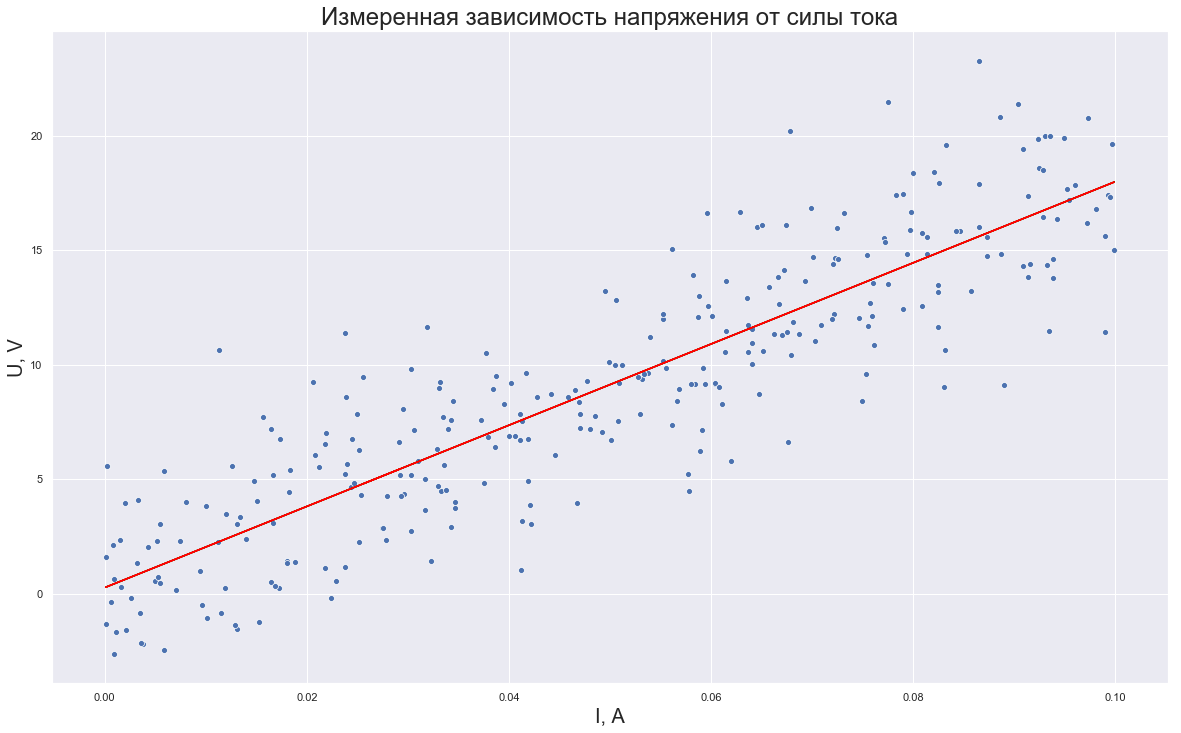
\includegraphics[width=\linewidth]{graphs/fig1.png}
\end{frame}

\begin{frame}{Ренессанс глубокого обучения в 2012 году}
    \pause{}
    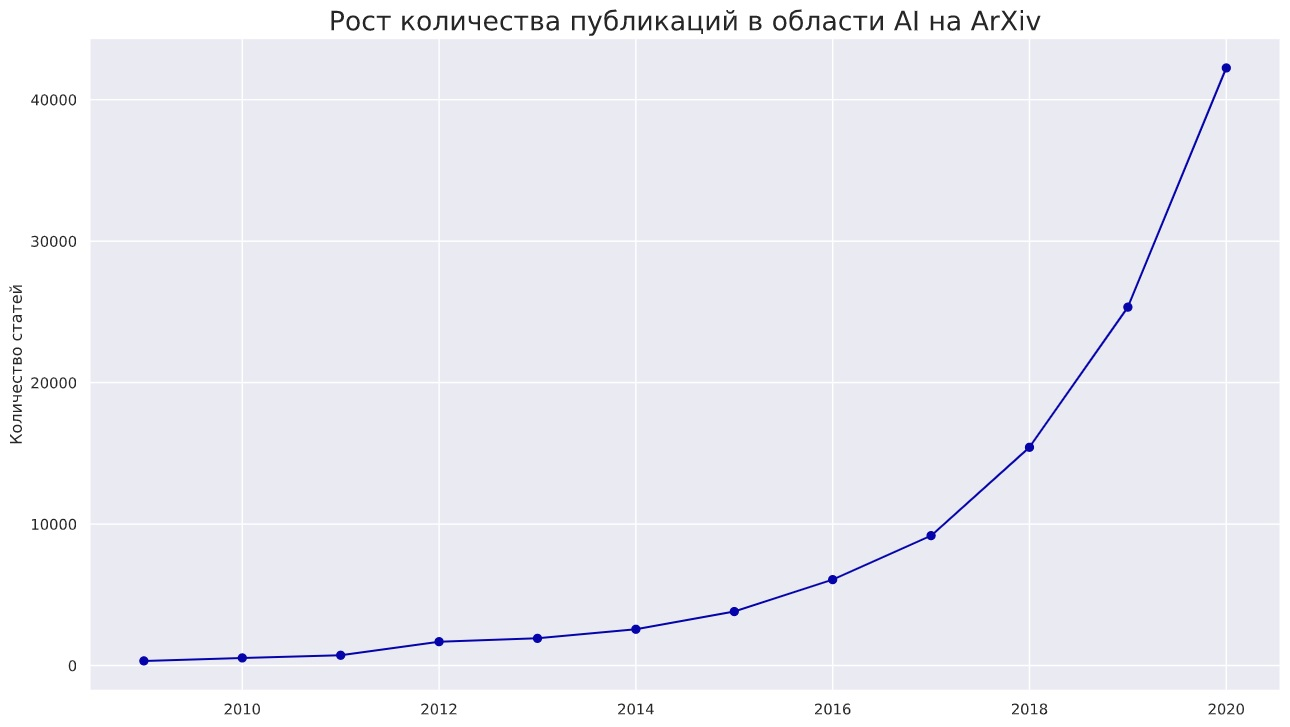
\includegraphics[width=\linewidth]{graphs/fig28.jpg}
\end{frame}

\begin{frame}{Ренессанс глубокого обучения в 2012 году}
    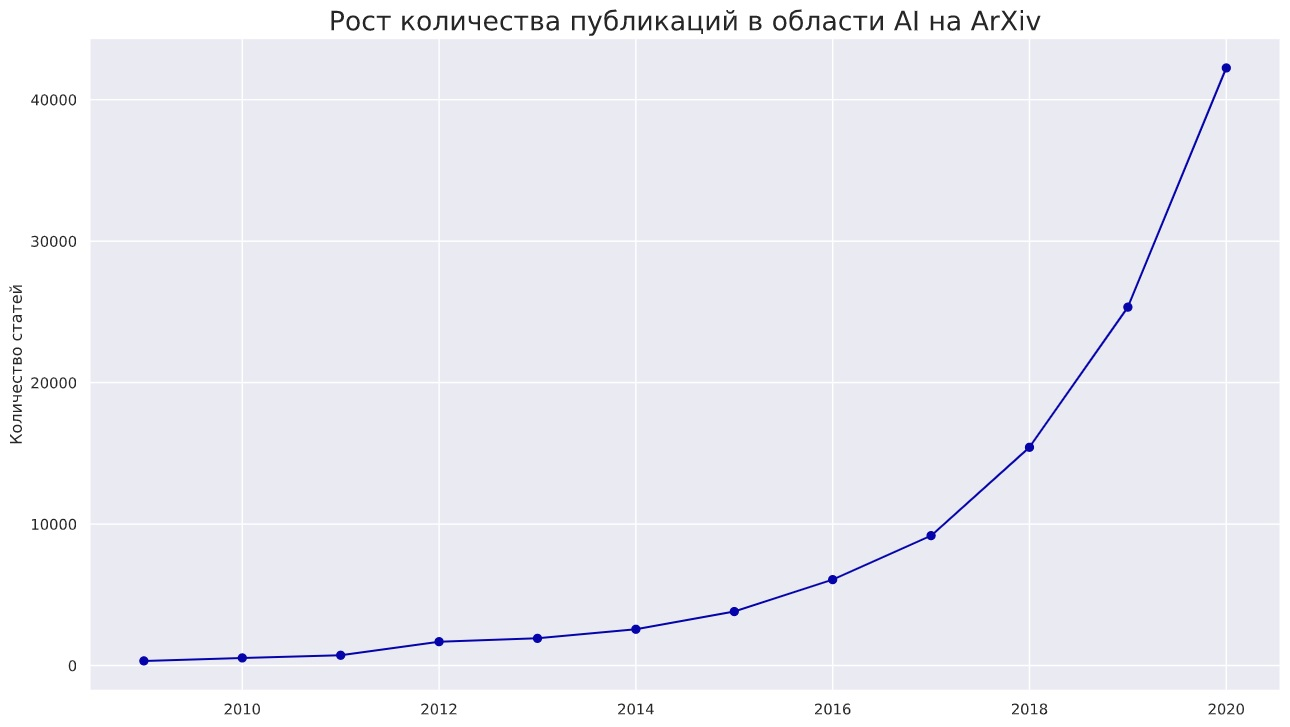
\includegraphics[width=0.95\linewidth]{graphs/fig29.png}
\end{frame}

\begin{frame}{Ренессанс глубокого обучения в 2012 году}
    \begin{itemize}
        \item C 2010 года проводится ILSVRC --- ImageNet Large Scale Visual
         Recognition Competition
        \item Это соревнование, помимо открытого доступа к большому датасету
         ImageNet, дало научному сообществу простой способ сравнивать
         различные модели
    \end{itemize}
\end{frame}

\begin{frame}{Ренессанс глубокого обучения в 2012 году}
    \pause{}
    \centering
    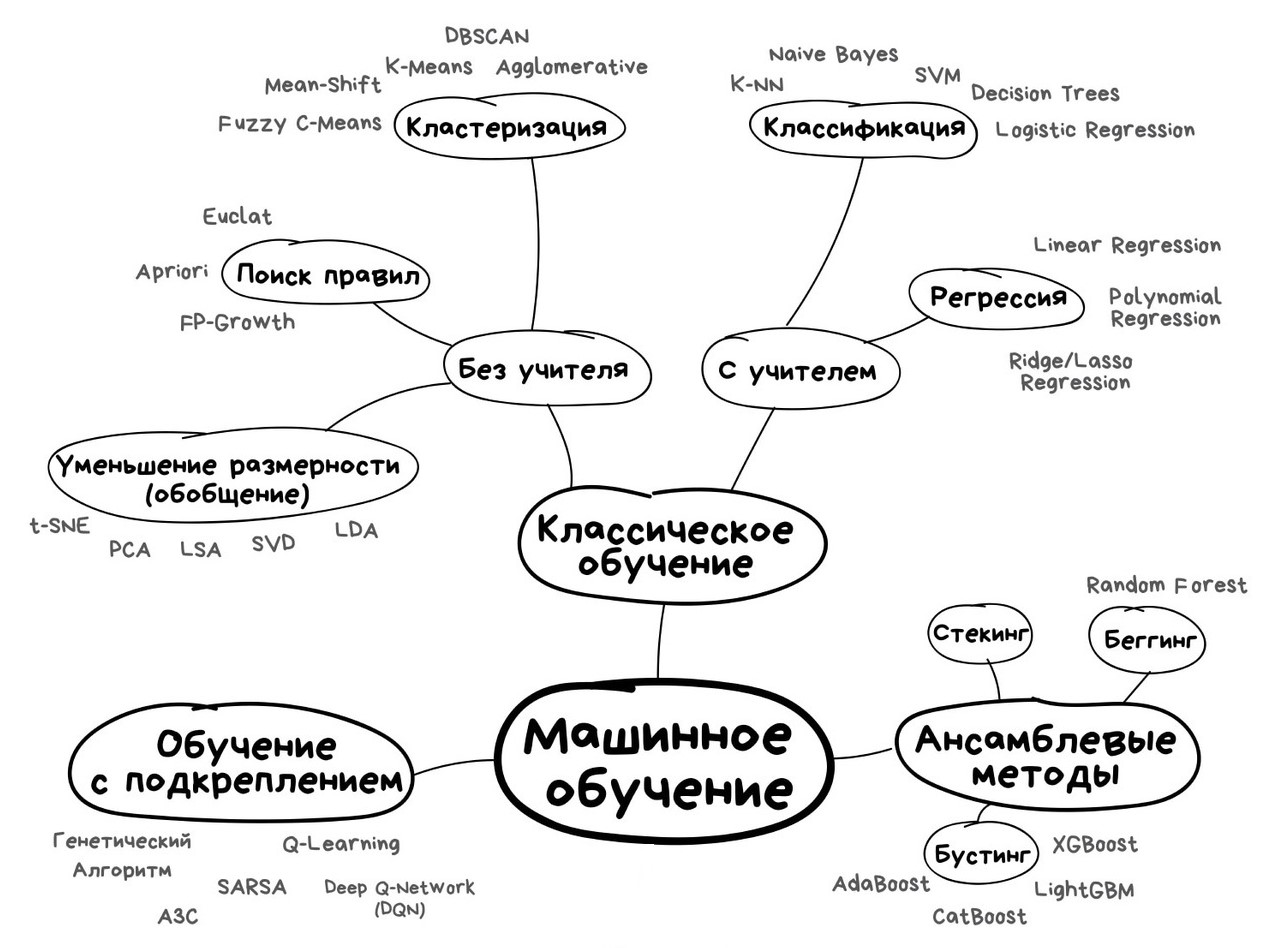
\includegraphics[width=0.74\linewidth]{graphs/fig30.jpg}
\end{frame}

\begin{frame}{Ренессанс глубокого обучения в 2012 году}
    \centering
    
\includegraphics[width=0.74\linewidth]{graphs/fig36.png}
\end{frame}

\begin{frame}{Начиная с 2012 года\ldots}
    \centering
    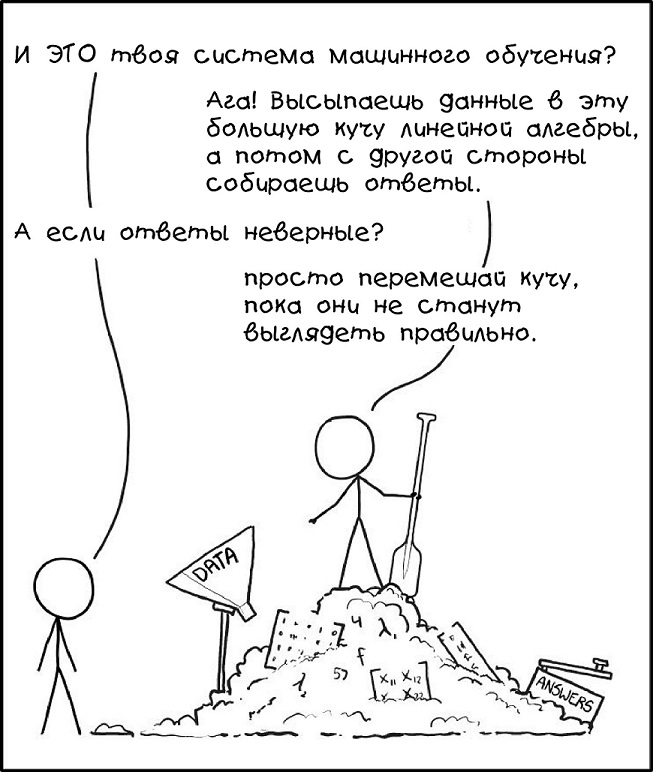
\includegraphics[width=0.63\linewidth]{graphs/fig37.png}
\end{frame}

\begin{frame}{Успех нейросетей}
    \centering
    \Large
    Успех нейросетей = \textbf{МНОГО} данных + \textbf{МНОГО} вычислительных
     мощностей
    \\
    Успех в классификации изображений = \textbf{ImageNet} + \textbf{GPUs}
\end{frame}

\begin{frame}{Как соотносятся между собой AI, ML, DL?}
    \centering
    \includegraphics[width=0.9\linewidth]{graphs/fig38.jpg}
\end{frame}

\begin{frame}{Задачи, которые решает машинное обучение}
    \centering
    \includegraphics[width=0.64\linewidth]{graphs/fig39.jpg}
\end{frame}

\begin{frame}{Задачи, которые решает машинное обучение}
    \centering
    \includegraphics[width=0.69\linewidth]{graphs/fig40.jpg}
\end{frame}

\begin{frame}{Задачи, которые решает машинное обучение}
    \centering
    \includegraphics[width=0.66\linewidth]{graphs/fig41.jpg}
\end{frame}

\begin{frame}{Важность задач классификации и регрессии}
    \begin{figure}
        \centering
        \includegraphics[width=0.6\linewidth]{graphs/fig44.jpg}
        \caption{Задача детектирования объектов (object detection)}
    \end{figure}
\end{frame}

\begin{frame}{Важность задач классификации и регрессии}
    \begin{figure}
        \centering
        \includegraphics[width=0.69\linewidth]{graphs/fig45.png}
        \caption{Задача семантической сегментации (semantic segmentation)}
    \end{figure}
\end{frame}

\begin{frame}{Как работает машинное обучение}
    \begin{figure}
        \begin{subfigure}[b]{0.49\linewidth}
            \includegraphics[width=0.67\linewidth]{graphs/fig42.jpg}
        \end{subfigure}
        \pause{}
        \begin{subfigure}[b]{0.49\linewidth}
            \includegraphics[width=0.79\linewidth]{graphs/fig43.png}
        \end{subfigure}
    \end{figure}
\end{frame}

\end{document}
